%% article.tex -- An article announcing Odum BASIC Simulations, for submission
%% to Ecological Modelling.

\documentclass[3p,times,authoryear,twocolumn]{elsarticle}

\journal{Ecological Modelling}

% --- Core Font & Encoding Packages ---
\usepackage[utf8]{inputenc}
\usepackage[T1]{fontenc}
\usepackage{lmodern}
\usepackage{microtype}

% --- Math, Physics & Graphics Packages ---
\usepackage{amsmath,amssymb}
\usepackage{graphicx}
\usepackage{subcaption}
\usepackage{tikz}
\usetikzlibrary{arrows.meta,calc,angles,quotes,decorations.markings,positioning}

% --- Tables, Code Listings & Formatting ---
\usepackage{booktabs}
\usepackage{tabularx}
\usepackage{listings}
\usepackage{xcolor}
\usepackage{framed}
\usepackage{comment}

% --- Hyperlinks (Load late) ---
\usepackage[hidelinks]{hyperref}

% --- Custom Commands ---
\newcommand{\gssk}{\textsc{gssk}}
\newcommand{\esl}{\textsc{esl}}
\newcommand{\idc}{\textsc{idc}}
\newcommand{\emsim}{\textsc{EmSim}}
\newcommand{\latexenergese}{\texttt{latex-energese}}
\newcommand{\code}[1]{\texttt{\small #1}}

% --- TikZ House Style ---
\tikzset{
  fluid/.style={fill=black!8},
  wall/.style={draw=black, thick},
  vel/.style={-{Latex[length=2.2mm]}, thick},
  thin vel/.style={-{Latex[length=1.8mm]}, semithick},
  dim/.style={|<->|, semithick},
  guide/.style={densely dashed, black!55},
  lbl/.style={font=\footnotesize},
}

% The figure goldens of the end-to-end suite (e2e/figures.spec.ts), and the screens
% of the oracle comparison (validation/oracle/screens.ts).
\graphicspath{{../e2e/figures/}{../validation/oracle/screens/}}

% The oracle comparison's numbers and table, generated by `make attest`.
%% Generated by validation/oracle/latex.ts from the attestation's runs. Do not edit:
%% run `make attest-update`, then review the diff. docs/article.tex \input's this file.

\newcommand{\oracleSteps}{640}
\newcommand{\oracleThresholdStep}{263}
\newcommand{\oracleThresholdT}{131.5}
\newcommand{\oracleSingleDoubleMaxRel}{$4.0\times10^{-5}$}
\newcommand{\oracleSingleDoubleMaxPx}{$6.8\times10^{-5}$}
\newcommand{\oracleDoubleMaxRel}{$3.7\times10^{-13}$}
\newcommand{\oracleBitIdenticalAssign}{22}
\newcommand{\oracleBitIdenticalEvery}{60}
\newcommand{\oracleReplaySteps}{639}
\newcommand{\oracleReplayDiffering}{466}
\newcommand{\oracleScreenPixels}{64{,}000}
\newcommand{\oracleScreenDiffering}{111}
\newcommand{\oracleEngineScreenDiffering}{111}
\newcommand{\oracleEnginesDiffering}{0}
\newcommand{\oraclePrecisionsDiffering}{0}
\newcommand{\oracleProbeValue}{0.5}
\newcommand{\oracleProbePset}{0}
\newcommand{\oracleProbeCint}{1}
\newcommand{\oraclePrintValues}{3{,}840}
\newcommand{\oraclePrintRoundedUp}{288}
\newcommand{\oraclePcbasicVersion}{2.0.8}
\newcommand{\oraclePythonVersion}{3.12.13}
\newcommand{\oracleNodeVersion}{26.5.1}

\newcommand{\oracleTable}{%
\begin{tabular}{@{}llccccc@{}}
\toprule
Runs & Arithmetic & \begin{tabular}[c]{@{}c@{}}Largest\\relative\\difference\end{tabular} & \begin{tabular}[c]{@{}c@{}}$D>30$\\from\\step\end{tabular} & \begin{tabular}[c]{@{}c@{}}Points on a\\different\\pixel\end{tabular} & \begin{tabular}[c]{@{}c@{}}Largest\\difference,\\pixels\end{tabular} & \begin{tabular}[c]{@{}c@{}}Steps\\bit-identical\\to R2\end{tabular} \\
\midrule
R1--R2 & ours, double vs.\ PC-BASIC, single & $4.0\times10^{-5}$ & 263 & 0 of 2{,}560 & $6.8\times10^{-5}$ & -- \\
R1--R3 & ours, double vs.\ PC-BASIC, \texttt{DEFDBL} & $3.8\times10^{-6}$ & 263 & 0 of 2{,}560 & $2.1\times10^{-6}$ & -- \\
R1--R3d & ours, double vs.\ PC-BASIC, double & $3.7\times10^{-13}$ & 263 & 0 of 2{,}560 & $5.7\times10^{-14}$ & -- \\
R2--R4a & PC-BASIC, single vs.\ ours, single on assignment & $4.4\times10^{-5}$ & 263 & 0 of 2{,}560 & $6.6\times10^{-5}$ & 22 of 640 \\
R2--R4b & PC-BASIC, single vs.\ ours, single throughout & $2.6\times10^{-5}$ & 263 & 0 of 2{,}560 & $6.6\times10^{-5}$ & 60 of 640 \\
\bottomrule
\end{tabular}}


\lstset{basicstyle=\ttfamily\footnotesize, columns=fullflexible, breaklines=true, frame=single, framesep=4pt, xleftmargin=6pt}

\begin{document}

% --- Front Matter Setup for elsarticle ---
\begin{frontmatter}

\title{A runtime for historical ecological simulation models written in BASIC}

\author{S. Maud\fnref{unsw}}
\ead{optional-email@unsw.edu.au}

\fntext[unsw]{University of NSW. \mbox{ORCID}: \href{https://orcid.org/0009-0004-1292-5980}{\mbox{0009-0004-1292-5980}}}

\begin{abstract}
Ecological simulation models published during the 1980s and 1990s frequently accompanied theoretical expositions as complete BASIC source code listings printed alongside Energy Systems Language diagrams. Although these publications provided full methodological disclosure, the obsolescence of underlying microcomputer architectures and proprietary BASIC dialects has rendered many of these historical models computationally inaccessible. In computational ecology, source code preservation alone does not guarantee long-term re-executability when the requisite execution environments decay. This paper presents Odum BASIC Simulations, an open-source execution runtime and archival framework designed to restore computational reproducibility to historical ecological models without modifying legacy source listings. The framework couples an in-browser execution engine supporting vintage Minimal BASIC and IBM PC graphics dialects with structured provenance validation conforming to research software preservation standards. The language core is implemented twice: an engine written in C, compiled to WebAssembly, which executes listings and checks them as they are edited, and an independent TypeScript interpreter retained as a reference implementation against which the engine is verified. Each model package integrates verified mathematical formulations, dialect fidelity classifications, and formal diagram attribution metadata. In numerical evaluations across representative benchmark models, the reconstructed runtime reproduced forward-Euler integration sequences to within floating-point display tolerances ($5\times10^{-7}$). Cross-platform comparative validation against an emulated historical execution environment demonstrated identical spatial rasterization across 2,560 trajectory coordinates, while resolving semantic discrepancies in midpoint pixel rounding via primary dialect source analysis. Agreement with an emulator constrains systematic error only insofar as the two implementations share no ancestry; the two independent implementations reported here, written in different languages and computing at different arithmetic precisions, reconstruct the published figure identically (\oracleEnginesDiffering{} differing pixels of \oracleScreenPixels{}), which tests that independence directly. The framework establishes a reproducible computational repository for systems ecology, providing a verified operational substrate for model inspection, validation, and historical reuse.
\end{abstract}

\begin{keyword}
systems ecology \sep H.T. Odum \sep Energy Systems Language \sep computational reproducibility \sep BASIC \sep software preservation \sep research software
\end{keyword}

\end{frontmatter}

%% ----------------------------------------------------------------------------
\section{Introduction}
\label{sec:intro}

Over a period of about 20 years, from 1980s-2000s, some systems ecologists published articles and books that contained two representations of quantitative dynamic simulation models: a conceptual Energy Systems Language (ESL) diagram (Fig.~\ref{fig:minimodel}), and the code for a computer simulation program (Fig.~\ref{fig:workbench}). This  convention was prominent in the works of Howard T. Odum, and persisted across multiple microcomputer generations culminating in instructional volumes that contained printed programs alongside software distributions on physical optical media \citep{odum1983,odumMinimodels,odumOdum2000}. The publication of complete listings provided an explicit operational specification of the underlying differential and difference equations of ecological and macroeconomic systems, enabling researchers and students to perform simulated hypothesis testing to evaluate transient trajectories and verify steady-state conditions directly on microcomputer hardware by altering coefficients.

Despite the convention of source code disclosure, the computational models of this period have largely become software artifacts in the archaeological record and unexecutable without excavatory effort involving the identification of an apprpirate runtime or software package. This is simply because the specialized microcomputer architectures for which the programs were compiled or interpreted have been retired from operational use, their associated software dialects have fragmented, and contemporary operating systems no longer provide compatible execution runtimes. 

\section{Software Collapse}
\label{sec:collapse}

The inability to execute these models today represents an impairment of scientific knowledge. Simulation models serve as formal instruments through which systems ecologists evaluate quantitative hypotheses regarding thermodynamic storage capacities, trophic cascades, and policy-driven regime shifts. While contemporary reproducibility initiatives frequently attribute replication failures to the omission of source code and advocate open code mandates \citep{peng2011,ince2012} or structured descriptive protocols \citep{grimm2010}, the decay of historical ecological models presents a distinct challenge. Complete source disclosures become computationally inert when their surrounding execution environments become obsolete, exemplifying the systemic phenomenon of \textit{software collapse} in scientific computing \citep{hinsen2019}.

In software engineering, operational obsolescence arising from external environmental divergence is recognized as a primary mode of software aging \citep{parnas1994}. However, standard software evolution literature predominantly examines continuous code modification within version-controlled repositories \citep{lehman1980,robles2005,spinellis2021}. Static printed listings occupy a divergent preservation regime: they remain immutable and structurally intact across decades, yet their semantic interpretation fails because the computational substrates that defined their execution no longer exist. Manual re-implementation into modern scientific programming languages partially mitigates this loss, but frequently introduces unrecorded translation artifacts, implicit algorithmic modifications, and undocumented transcription discrepancies.

\section{The Case of H.T. Odum}
\label{sec:odum}

As a case in point, in the historical period of interest for this article, H.T.Odum published ecological models using a dialect of the BASIC programming language. Unfortunately, modern operating systems no longer include built-in interpreters (like QBasic or GW-BASIC from early DOS days) for this dialect. Currently supported Windows Operating System shells---Command terminal and PowerShell (and Macos/Linux Bash terminal)---do not natively support or execute the dialect of of Odum's BASIC programs. These shells interpret their own specific command/scripting languages but not BASIC, and consequently the published BASIC ecological models of the 1980-2000s cannot be directly evaluated against their originally published quantitative trajectories, compared systematically with alternative formulations, or integrated into modern ecological research workflows.

The argument motivating the present paper and associated efforts says that this loss of computational runtime environment impairs an important aspect of the scientific method: repeatability. And without repeatability, human epistemology cannot consolidate around a shared ontology. As a result, the epistemological utility of such models depends on independent computational reproducibility, as originally intended by the open publication of their source listings. Verification, falsification, validation of these programs in computational ecological modeling represents an important step in the debates around the foundational public claims of systems ecologists regarding the concepts of climate change and peak oil that being made in this period and which are being questioned by an organised international community of climate skeptics and radical boursgeioe anti-woke activists who consider the word `ecology' to be a DEI limitation of capitalism. 

\section{Case Study: Macro-Ecologic-Economic Minimodel}
\label{sec:case:study}

\begin{figure}[tb]
  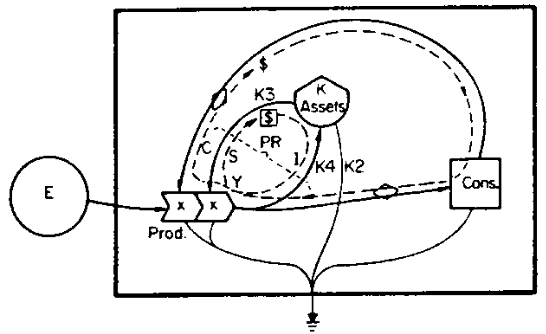
\includegraphics[width=\linewidth]{./images/macro_economic.png}
  \caption{``Simple macro-ecologic-economic minimodel to demonstrate  methods of diagramming and simulation'' \cite[fig.~2a, p.~71]{odum1989}}
\end{figure}

\begin{figure}[tb]
  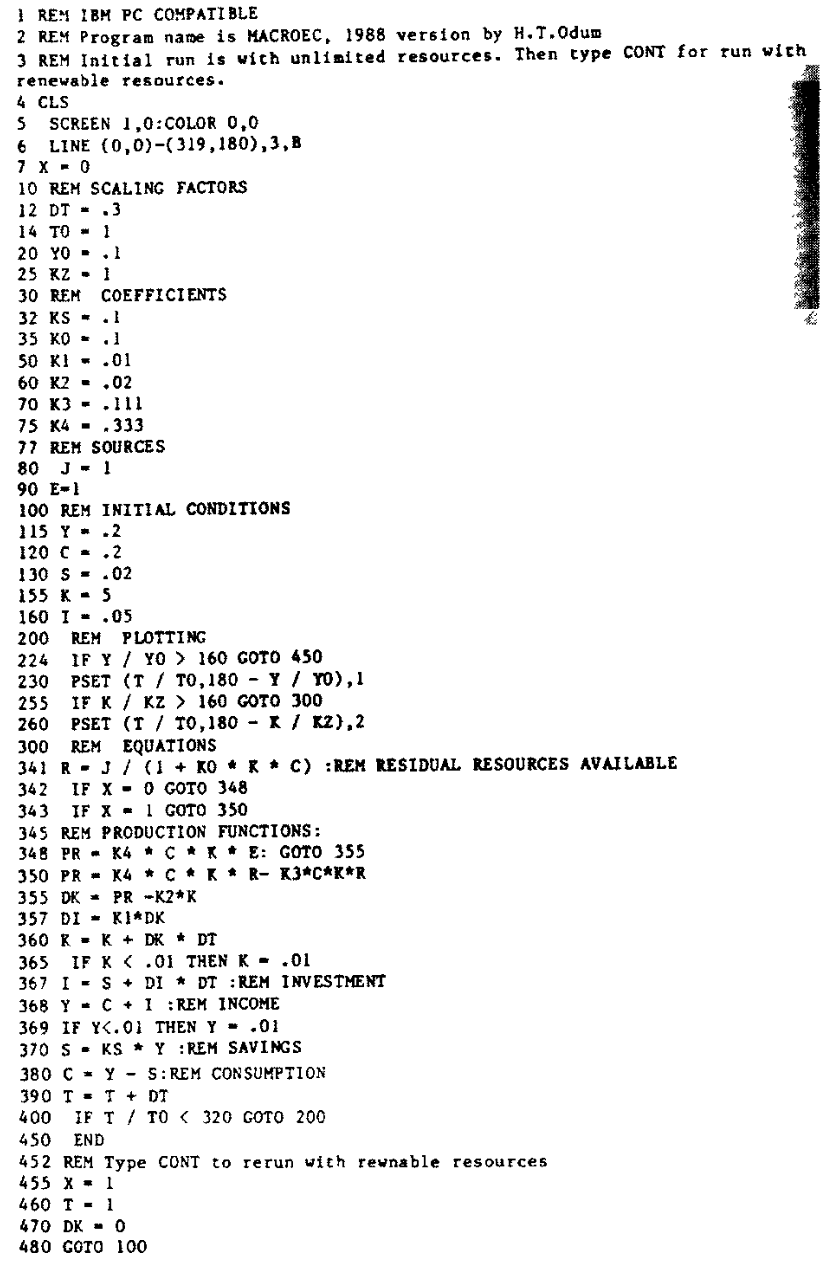
\includegraphics[width=\linewidth]{./images/macro_economic_basic.png}
  \caption{``BASIC PC Microcomputer Simulation Program for  the Macroeconomics Minimodel'' \cite[table.~2, p.~71]{odum1989}}
  \label{fig:macroec:basic}
\end{figure}


\subsection{What ``modernizing'' a listing involves}
\label{sec:case:modernize}

The obvious alternative to a dedicated runtime is to translate a listing into a language that current systems still execute. The usual recipe for doing so is short: strip out the line numbers, drop the legacy \texttt{LET} keyword, wrap the executable statements in a \texttt{Sub Main()} subroutine, and replace BASIC's \texttt{PRINT} statements with formatted console output. Listing~\ref{lst:macroec} is MACROEC as Odum printed it (Figure~\ref{fig:macroec:basic}), transcribed line for line; Listing~\ref{lst:macroec:vb} is the Visual Basic .NET module the recipe leads to, once the gaps it leaves have been filled.

\begin{lstlisting}[basicstyle=\ttfamily\scriptsize,keepspaces=true,caption={MACROEC, transcribed from Figure~\ref{fig:macroec:basic} {\citep[Table~2]{odum1989}}. The scan's typeface does not distinguish the letter O from the digit zero; \texttt{T0}, \texttt{Y0} and \texttt{K0} are read as zeros, since \texttt{TO} is a reserved word and each name is assigned before it is used. The misspelling in line 452 is Odum's.},label={lst:macroec}]
1 REM IBM PC COMPATIBLE
2 REM Program name is MACROEC, 1988 version by H.T.Odum
3 REM Initial run is with unlimited resources. Then type CONT for run with renewable resources.
4 CLS
5  SCREEN 1,0:COLOR 0,0
6  LINE (0,0)-(319,180),3,B
7 X = 0
10 REM SCALING FACTORS
12 DT = .3
14 T0 = 1
20 Y0 = .1
25 KZ = 1
30 REM  COEFFICIENTS
32 KS = .1
35 K0 = .1
50 K1 = .01
60 K2 = .02
70 K3 = .111
75 K4 = .333
77 REM SOURCES
80  J = 1
90 E=1
100 REM INITIAL CONDITIONS
115 Y = .2
120 C = .2
130 S = .02
155 K = 5
160 I = .05
200  REM  PLOTTING
224  IF Y / Y0 > 160 GOTO 450
230  PSET (T / T0,180 - Y / Y0),1
255  IF K / KZ > 160 GOTO 300
260  PSET (T / T0,180 - K / KZ),2
300  REM  EQUATIONS
341 R = J / (1 + K0 * K * C) :REM RESIDUAL RESOURCES AVAILABLE
342  IF X = 0 GOTO 348
343  IF X = 1 GOTO 350
345 REM PRODUCTION FUNCTIONS:
348 PR = K4 * C * K * E: GOTO 355
350 PR = K4 * C * K * R- K3*C*K*R
355 DK = PR -K2*K
357 DI = K1*DK
360 K = K + DK * DT
365  IF K < .01 THEN K = .01
367 I = S + DI * DT :REM INVESTMENT
368 Y = C + I :REM INCOME
369 IF Y<.01 THEN Y = .01
370 S = KS * Y :REM SAVINGS
380 C = Y - S:REM CONSUMPTION
390 T = T + DT
400  IF T / T0 < 320 GOTO 200
450  END
452 REM Type CONT to rerun with rewnable resources
455 X = 1
460 T = 1
470 DK = 0
480 GOTO 100
\end{lstlisting}

\begin{lstlisting}[basicstyle=\ttfamily\scriptsize,keepspaces=true,caption={Listing~\ref{lst:macroec} ``modernized'' into a Visual Basic .NET module. Everything the recipe does not cover---the graphics, the \texttt{GOTO} structure, the \texttt{CONT} restart---had to be decided by the translator.},label={lst:macroec:vb}]
' MACROEC, 1988 version by H.T. Odum.
' Initial run is with unlimited resources,
' then a run with renewable resources.
Module Macroec
  Sub Main()
    Dim DT As Double = 0.3, T0 As Double = 1
    Dim Y0 As Double = 0.1, KZ As Double = 1
    Dim KS As Double = 0.1, K0 As Double = 0.1
    Dim K1 As Double = 0.01, K2 As Double = 0.02
    Dim K3 As Double = 0.111, K4 As Double = 0.333
    Dim J As Double = 1, E As Double = 1
    Dim Y, C, S, K, I, R, PR, DK, DI As Double
    Dim T As Double = 0
    For X As Integer = 0 To 1
      ' Initial conditions
      Y = 0.2 : C = 0.2 : S = 0.02 : K = 5 : I = 0.05
      Console.WriteLine("{0,8}{1,10}{2,10}", _
        "T", "Y", "K")
      Do
        If Y / Y0 > 160 Then Exit Do
        Console.Write("{0,8:N1}{1,10:N4}", T, Y)
        If K / KZ <= 160 Then
          Console.Write("{0,10:N4}", K)
        End If
        Console.WriteLine()
        ' Equations
        R = J / (1 + K0 * K * C)  ' residual resources
        If X = 0 Then
          PR = K4 * C * K * E
        Else
          PR = K4 * C * K * R - K3 * C * K * R
        End If
        DK = PR - K2 * K
        DI = K1 * DK
        K = K + DK * DT
        If K < 0.01 Then K = 0.01
        I = S + DI * DT           ' investment
        Y = C + I                 ' income
        If Y < 0.01 Then Y = 0.01
        S = KS * Y                ' savings
        C = Y - S                 ' consumption
        T = T + DT
      Loop While T / T0 < 320
      If X = 0 Then
        Console.Write("Press Enter to rerun with ")
        Console.WriteLine("renewable resources.")
        Console.ReadLine()
        T = 1
      End If
    Next X
  End Sub
End Module
\end{lstlisting}

The result compiles and runs, and its equations are those of the published listing. It is nonetheless a different program. Table~\ref{tab:modernize} records where it departs from the published text, and every departure is a decision the translator made on the author's behalf that no reader comparing the output with the 1989 article can check against the page.

\begin{table*}[t]
\centering\small
\begin{tabularx}{\linewidth}{@{}p{0.27\linewidth}p{0.25\linewidth}X@{}}
\toprule
Original BASIC (Listing~\ref{lst:macroec}) & Visual Basic .NET (Listing~\ref{lst:macroec:vb}) & Consequence \\
\midrule
\texttt{1 REM ...} & \texttt{' ...} & None: comment syntax only. \\
\texttt{12 DT = .3} & \texttt{Dim DT As Double = 0.3} & Single-precision arithmetic silently becomes double precision. \\
\texttt{4 CLS}, \texttt{5 SCREEN 1,0}, \texttt{6 LINE (0,0)-(319,180),3,B} & omitted & A console has no graphics mode; the framed $320\times180$ plot has nowhere to go. \\
\texttt{230 PSET (T / T0,180 - Y / Y0),1} and \texttt{260 PSET ...,2} & \texttt{Console.Write(...)} & The figure the program exists to draw becomes a table in a format the translator chose. Rounding each point to a pixel, which decides what the published figure shows, disappears. \\
\texttt{200}--\texttt{400}: a loop built from \texttt{GOTO}s & \texttt{Do ... Loop While} & The control flow is restructured to the translator's reading of the jumps, including the early exit at line 224 and the skipped point at line 255. \\
\texttt{450 END}, then \texttt{CONT} at the keyboard, \texttt{452}--\texttt{480} & \texttt{For X = 0 To 1}, \texttt{Console.ReadLine()} & Resuming a program after \texttt{END} is a facility of the GW-BASIC interpreter, not of any compiled language; the second experiment is re-expressed as a loop the author never wrote. \\
\bottomrule
\end{tabularx}
\caption{The changes made by the ``modernization'' of Listing~\ref{lst:macroec} into Listing~\ref{lst:macroec:vb}, and what each does to the program.}
\label{tab:modernize}
\end{table*}

Only the first row is the cosmetic change the recipe promises. Declaring the variables \texttt{Double} changes the arithmetic: GW-BASIC variables are single precision unless declared otherwise, so the translated program integrates the same equations to about fifteen significant digits where the original carried about seven. Because $0.3$ is not exactly representable in binary, $T$ accumulates rounding differently at the two precisions over the thousand-odd steps of each run, and whether the last step before $T/T_0$ reaches 320 is taken can differ between them. The recipe's central instruction, to replace \texttt{PRINT} with formatted output, has no purchase on MACROEC at all: the program never prints. It draws income and assets point by point on a CGA screen, and the translation can only substitute a table for the figure. Its second experiment is reached interactively: line 450 ends the run with unlimited resources, the reader types \texttt{CONT}, and execution resumes at line 452 with renewable resources, which a translator can only imitate by inventing a mechanism of their own.

Nor does translation escape the problem it sets out to solve. The recipe's two routes to execution are the \texttt{vbc.exe} compiler of the .NET Framework and, to avoid compiling, running the program as VBScript under Windows Script Host's \texttt{cscript}. Both are Windows-only, and VBScript is on Microsoft's own list of deprecated Windows features.\footnote{\url{https://learn.microsoft.com/en-us/windows/whats-new/deprecated-features}} Translation moves a listing from one decaying runtime to another, and gives up its correspondence with the printed page on the way.

To address these limitations, this paper introduces Odum BASIC Simulations, an open-access archival framework and execution runtime designed to recover the repeatability of historical ecological simulations. Rather than translating legacy code into contemporary frameworks, the system reconstructs an execution environment tailored to the original source text, formalizing the relationship between the printed historical artifact and its modern execution as machine-checked provenance data. 

This article is undertaken under a broader research program documented as one of has four pillars in the Energese-Project GitHub Organisation. The pillars are: latex-energese, a package for latex publishing to support the Energy Systems Language; GSSK, a simulation kernel for supporting energy systems dynamics, emergy algorithms and Giannantoni's incipient calculus, GSSK-Dia, a diagrammatic interface for constructing valid GSSK systems models and Odum-BASIC-Simulations, the subject of this article.

the preservation of historical ecological models, which encompasses the formalization of Energy Systems Language diagrammatic syntax \citep{energese}, the development of a web-based interactive workbench for model inspection and execution, and the establishment of structured metadata schemas for archival fidelity. The present study focuses on the design, implementation, and verification of a runtime capable of executing legacy BASIC listings in a manner faithful to their original semantics. 


This study presents four primary contributions:
\begin{enumerate}
% RESOLVED(contributions): contribution 1 names both implementations and says
% what the second one buys; contribution 4 names independent reimplementation
% as a verification method alongside the emulator comparison.
\item \textbf{A reconstructed execution runtime, implemented twice:} A client-side engine designed to execute legacy ecological BASIC listings without source code alteration, providing tabular data extraction from sequential console outputs and coordinate rasterization for graphical trajectory statements. The language core exists in two independent realizations --- an engine in C, compiled both to WebAssembly and to a native command-line executable, and an interpreter in TypeScript --- which is what makes the verification in contribution~4 possible.
\item \textbf{An evidential ranking protocol:} A structured framework for arbitrating semantic conflicts among historical specifications, primary interpreter source code, original manuals, and contemporary emulators.
\item \textbf{A machine-validated provenance ontology:} An archival metadata specification enforcing explicit provenance, rights statements, and dialect fidelity classifications compliant with FAIR4RS guidelines \citep{barker2022}.
\item \textbf{A rigorous verification methodology:} A systematic evaluation framework incorporating exact analytical benchmarks, automated regression harnesses, cross-runtime pixel-level comparisons against emulated historical interpreters, and agreement between two independently written implementations of the language core computing at different arithmetic precisions.
\end{enumerate}

%% ----------------------------------------------------------------------------
\section{Background: simulation in Odum's systems ecology}
\label{sec:background}

The Energy Systems Language was initially conceived through formal analogies between ecosystem mass-energy flows and electrical network potentials, wherein compartmental storages operate analogously to capacitors and energetic transfers represent flow currents \citep{odum1960}. Over subsequent decades, this conceptualization matured into a macroscopic modeling formalization, employing standardized symbols for energy sources, state storages, multiplicative interactions, autotrophic producers, heterotrophic consumers, and dispersed heat sinks \citep{odum1972,odum1983,odum1994}. Mathematical simulation formed an integral component of the formalization. Each graphical diagram mathematically defines a coupled system of first-order ordinary differential equations, which were historically resolved on analog computing hardware before transitioning to numerical integration on laboratory microcomputers during the 1980s. The formal typography of the visual language is addressed in companion work \citep{energese}; the present investigation focuses on the execution fidelity of the corresponding numerical models.

The selection of BASIC as the computational medium for systems ecology models reflected the technical affordances of early microcomputing. Developed originally to facilitate algorithmic instruction without the overhead of complex toolchains \citep{kemenyKurtz1964}, dialect implementations became ubiquitous across personal microcomputers. For published ecological literature, short interpreted listings offered an accessible mechanism for mathematical dissemination. 

\begin{lstlisting}[caption={Representative structural syntax of an ecological simulation listing, illustrating state initialization, forward-Euler numerical integration, and sequential state output.},label={lst:shape}]
100 LET J = 100
110 LET K1 = 0.1
120 LET Q = 0
130 LET DT = 0.5
140 PRINT "T", "Q", "OUTFLOW"
150 FOR T = 0 TO 60 STEP DT
160 LET F = K1 * Q
170 PRINT T, Q, F
180 LET Q = Q + (J - F) * DT
190 NEXT T
\end{lstlisting}

Historical listings across this literature exhibit consistent structural patterns, as exemplified in Listing~\ref{lst:shape}. Model parameters, temporal discretizations, and initial state storages are initialized via explicit assignments; a bounded iterative loop advances simulation time by constant increments of \texttt{DT}; compartmental fluxes are calculated from instantaneous state magnitudes; storages are updated via explicit forward-Euler numerical integration; and output values are periodically reported via sequential print statements or dedicated graphics commands. Two primary dialect families characterize this literature: early implementations adhering closely to the Minimal BASIC standard core \citep{ecma55}, and subsequent PC-DOS implementations incorporating hardware-specific display commands (\texttt{SCREEN}, \texttt{PSET}, and \texttt{LINE}) to plot dynamic phase trajectories directly on the display screen \citep{odum1989}.

Current computational approaches remain inadequate for the preservation of these historical models. While general hardware emulators can execute legacy software environments, they introduce significant operational friction: they require proprietary firmware ROM images that cannot be distributed in open scholarly repositories, reproduce hardware-level abstractions rather than model-level representations, and lack mechanisms for structured provenance tracking. Conversely, re-encoding these models in contemporary general-purpose system dynamics environments \citep{richmond1985,fortmannRoe2014,vensim} requires reformulating the original source text, introducing silent discrepancies between the archival literature and the executing artifact. Historical web distributions of pedagogical ecological models \citep{ortega2007} have preserved accompanying descriptive texts but remain static, leaving the models unexecutable.

In digital preservation and software archaeology, empirical investigations typically analyze version-control lineages to assess developer turnover, architectural drift, and component survival \citep{huntThomas2002,robles2005,spinellis2021}. These analytical models presume continuous software evolution across active development cycles. In contrast, published ecological program listings represent static, immutable artifacts that possess neither version-control histories nor ongoing maintenance cycles. The underlying source text remains unchanged, but the operational environment has disintegrated. Consequently, restoring computational repeatability requires reconstructing the execution runtime around the original textual artifact, establishing an evidential basis for historical language semantics while linking program provenance directly to archival literature.

Modern research software preservation frameworks, including the FAIR4RS principles \citep{barker2022} and formal software citation standards \citep{smith2016}, emphasize findability, accessibility, interoperability, and reusability. However, these criteria evaluate software artifacts under the assumption that the preservation object is self-contained and natively runnable. For historical transcriptions, preservation schemas must also incorporate an explicit metric of transcription fidelity, quantifying the structural correspondence between the executed code and the published historical record.

%% ----------------------------------------------------------------------------
\section{Design principles and architectural criteria}
\label{sec:design}

The development of the preservation framework was governed by five methodological criteria designed to ensure archival integrity and numerical reliability:

\paragraph{Invariance of the historical artifact} The primary source listing constitutes the immutable scientific object. If an incompatibility arises between a published historical listing and the execution runtime, the deficiency is attributed to the interpreter rather than the source text. Legacy source listings are not modified or modernized. Output trajectories are extracted directly from the formatting structures emitted by the original program, whether through tabular console streams or screen-space graphics primitives. Unimplemented dialect operations are cataloged as runtime limitations rather than accommodated via intrusive code alterations.

\paragraph{Machine-enforceable provenance schemas} Computational reproducibility requires transparent pedigree tracking. Every archived program is coupled with a structured metadata specification file. The build pipeline enforces schema validation, rejecting any submission characterized by missing bibliographic properties, invalid relational identifiers, or undefined fidelity classifications. 

\begin{table*}[t]
\centering\small
\begin{tabularx}{\linewidth}{@{}lXp{0.34\linewidth}@{}}
\toprule
Fidelity level & Definition & Required metadata \\
\midrule
\texttt{verbatim} & Character-for-character transcription of the published source, including typographical errata & Bibliographic source citation \\
\texttt{corrected} & Transcription containing minimal corrections of verified typographical errors & Bibliographic citation; itemized mutation list \\
\texttt{adapted} & Algorithmic reconstruction or substantial modernization of a published model & Bibliographic source citation \\
\texttt{original} & Independent benchmark model authored specifically for runtime verification & Archival description \\
\bottomrule
\end{tabularx}
\caption{Taxonomy of program fidelity classifications implemented within the preservation framework.}
\label{tab:fidelity}
\end{table*}

The metadata schema defines four discrete tiers of transcription fidelity (Table~\ref{tab:fidelity}). The assignment of fidelity levels requires explicit human adjudication based on physical source verification; automated workflows are prohibited from establishing or mutating this parameter.

\paragraph{Hierarchical evidentiary ordering} Determining historical execution semantics requires reconciling divergent technical documentation. When behavioral discrepancies arise between reference sources, evidence is arbitrated through a strict hierarchical ranking:
\begin{enumerate}
\item Formal consensus standards, including Standard ECMA-55 for Minimal BASIC \citep{ecma55}.
\item Primary source implementations, specifically the released source code of original historical interpreters \citep{gwbasic}.
\item Contemporary technical reference manuals issued by original compiler vendors.
\item Independent modern emulators and secondary reconstructions \citep{pcbasic}.
\end{enumerate}
Where modern emulators deviate from primary interpreter source code, the framework conforms to the primary source implementation, documenting the discrepancy as a known divergence within the validation record.

% RESOLVED(design/longevity): the paragraph now states the committed-artefact
% case and the rebuild check that keeps it honest (engine/build-wasm.sh
% --check, the `wasm` job).
\paragraph{Architectural longevity and independence} To prevent the recurrence of software collapse, the runtime is constructed entirely on open, standardized web platform primitives without reliance on transient server-side infrastructure, remote databases, or dynamic content-delivery network dependencies. All runtime libraries and architectural components are vendored directly within the static repository structure, ensuring that the archive remains fully functional as a self-contained computational distribution. This extends to compiled artifacts: the WebAssembly build of the execution engine is committed to the repository, because the deployment runner provides neither a C toolchain nor a container runtime, and an archive that can only be built on a machine with the right compiler installed has merely relocated the dependency it was trying to remove. A committed binary can silently cease to correspond to its source, so continuous integration rebuilds it within a digest-pinned toolchain image on every proposed change and fails if a single byte differs. The longevity principle is thereby applied to build products as well as to source: what is archived is executable without reconstruction, and what is executable is provably derived from what is archived.

\paragraph{Behavioral, specification-first test harnesses} System modifications are validated through external behavioral assertions rather than unit-level internal state tests. Interpreter test suites execute concrete BASIC listings and evaluate rendered output tables, while archival validation harnesses ensure metadata completeness, bibliographic integrity, and asset compliance.

%% ----------------------------------------------------------------------------
\section{Runtime architecture and execution engine}
\label{sec:implementation}

% RESOLVED(implementation): the section now describes both implementations and
% which one executes. NOTE for anyone reading the marker this replaced: it was
% written at 56a43e8 and its last bullet had gone stale. INPUT is implemented
% (BAS_AWAITING_INPUT, a status that is neither success nor failure), PRINT
% produces the console's text (BAS_TakeText), and SCREEN/COLOR/CLS are recorded,
% so execution moved to the C engine and the site no longer runs the TypeScript
% interpreter at all. The roles are the reverse of what the marker assumed.
The language core is implemented twice, independently, and neither implementation depends on an external machine emulator or on proprietary binary firmware. The implementation that executes listings is written in C and compiled from a single source to two targets: a WebAssembly module shipped with the site, and a native command-line executable providing \texttt{run} and \texttt{check} subcommands. The second implementation is an interpreter in TypeScript, which executed listings in earlier releases and is now retained as a reference implementation: it is the independent second opinion the verification in Section~\ref{sec:validation} rests on, and is exercised by its own test suite rather than by the site.

Separating checking from running is deliberate and is reflected in the engine's interface. Validation parses and analyzes a listing without executing any part of it, which makes it safe to invoke on every keystroke in the editor; execution is driven in bounded slices, running at most a specified number of statements per call, so that a supervising Web Worker retains the ability to halt a program that does not terminate, and so that \texttt{CONT} can resume from the program counter at which \texttt{END} or \texttt{STOP} left it. Suspension is a first-class outcome rather than an error: an \texttt{INPUT} statement returns a distinct status meaning that a line of input is awaited, which is neither success nor failure, and the same mechanism carries the resumption.

A further consequence of this design is that the engine emits graphical output as rows in the program's own coordinate space and never as pixels. Rasterization is performed by a separate routine shared with the TypeScript interpreter, which is precisely what permits the comparison in Section~\ref{sec:validation}: because both implementations are rasterized by the same code, any difference between their screens must originate in the arithmetic rather than in the drawing.

Both implementations cover the language core required by historical systems ecology models: standard numeric and string variables, multi-dimensional arrays declared via \texttt{DIM}, conditional statements (\texttt{IF/THEN}), branching and subroutine mechanics (\texttt{GOTO}, \texttt{GOSUB/RETURN}), sequential input/output primitives (\texttt{PRINT}, \texttt{INPUT}, \texttt{DATA/READ/RESTORE}), loop constructs (\texttt{FOR/TO/STEP/NEXT}), and fundamental mathematical functions including \texttt{EXP}, \texttt{LOG}, \texttt{SQR}, \texttt{INT}, and \texttt{RND}.

For later PC-DOS listings, both implementations provide the standard graphics operations, including \texttt{SCREEN} modes 1 and 2, \texttt{COLOR}, \texttt{CLS}, and the drawing statements (\texttt{PSET}, \texttt{PRESET}, and \texttt{LINE} with coordinate offsets and box-fill parameters), alongside resumption of execution via \texttt{CONT}. The display-configuration statements are recorded in the output stream rather than discarded, because a rasterizer cannot size a buffer until it knows the mode that was selected; the stream is therefore an ordered record of everything a listing emitted, not only of the points it plotted. Downstream of that stream, two representations are maintained: coordinates are rasterized to an emulated display buffer, reproducing the screen as the original hardware showed it, and are simultaneously retained as continuous numerical vectors in the program's own units, enabling analytical trajectory recovery. Keeping these apart matters for the comparisons in Section~\ref{sec:validation}: the pixels are how a run appeared, which is what published figures record, whereas the vectors are what it computed. Structured control operations and complex formatting statements that are absent from early ecological listings are parsed and styled within the interface as pending language features.

% RESOLVED(implementation/precision): the paragraph now names which
% implementation each claim describes, and states the engine's compile-time
% arithmetic contract. See engine/include/basic_config.h, which argues both
% hazards out. What is still missing from this section is the rest of the
% architecture -- REVIEW(implementation) above -- not the precision.
Numerical computation in the TypeScript interpreter is conducted in IEEE-754 double-precision floating-point arithmetic, with tabular console output formatted to six decimal places. The C engine, which is the implementation the site now executes, computes in IEEE-754 single precision: \texttt{BAS\_Real} is C's \texttt{float}, so every operation rounds to single because that is what the type does, and its console output gives a single seven significant digits as GW-BASIC did. That contract is enforced at compile time rather than assumed --- the build requires \texttt{FLT\_EVAL\_METHOD == 0} and refuses to compile without it, since evaluating intermediates more widely would turn \texttt{A = A + DA * DT} into one rounding where GW-BASIC performed three, and \texttt{-ffp-contract=off} is passed because a fused multiply-add rounds once where the original rounded twice. Historical microcomputer interpreters utilized shorter numerical formats; for example, Commodore BASIC V2 employed a 5-byte format (32-bit significand, 8-bit exponent) yielding approximately nine decimal digits, whereas GW-BASIC implemented 4-byte single-precision Microsoft Binary Format (MBF) yielding approximately seven significant digits. Consequently, runtime fidelity is calibrated to reproduce the underlying compartmental model equations and dynamic trajectories, while recognizing that the least significant printed digits may reflect architectural precision differences. Execution proceeds within an isolated Web Worker thread, maintaining responsiveness and preventing the interface from freezing during iterative numerical integration loops; because the engine executes in bounded slices, a non-terminating listing can be interrupted rather than merely waited out.

\begin{figure*}[t]
\centering
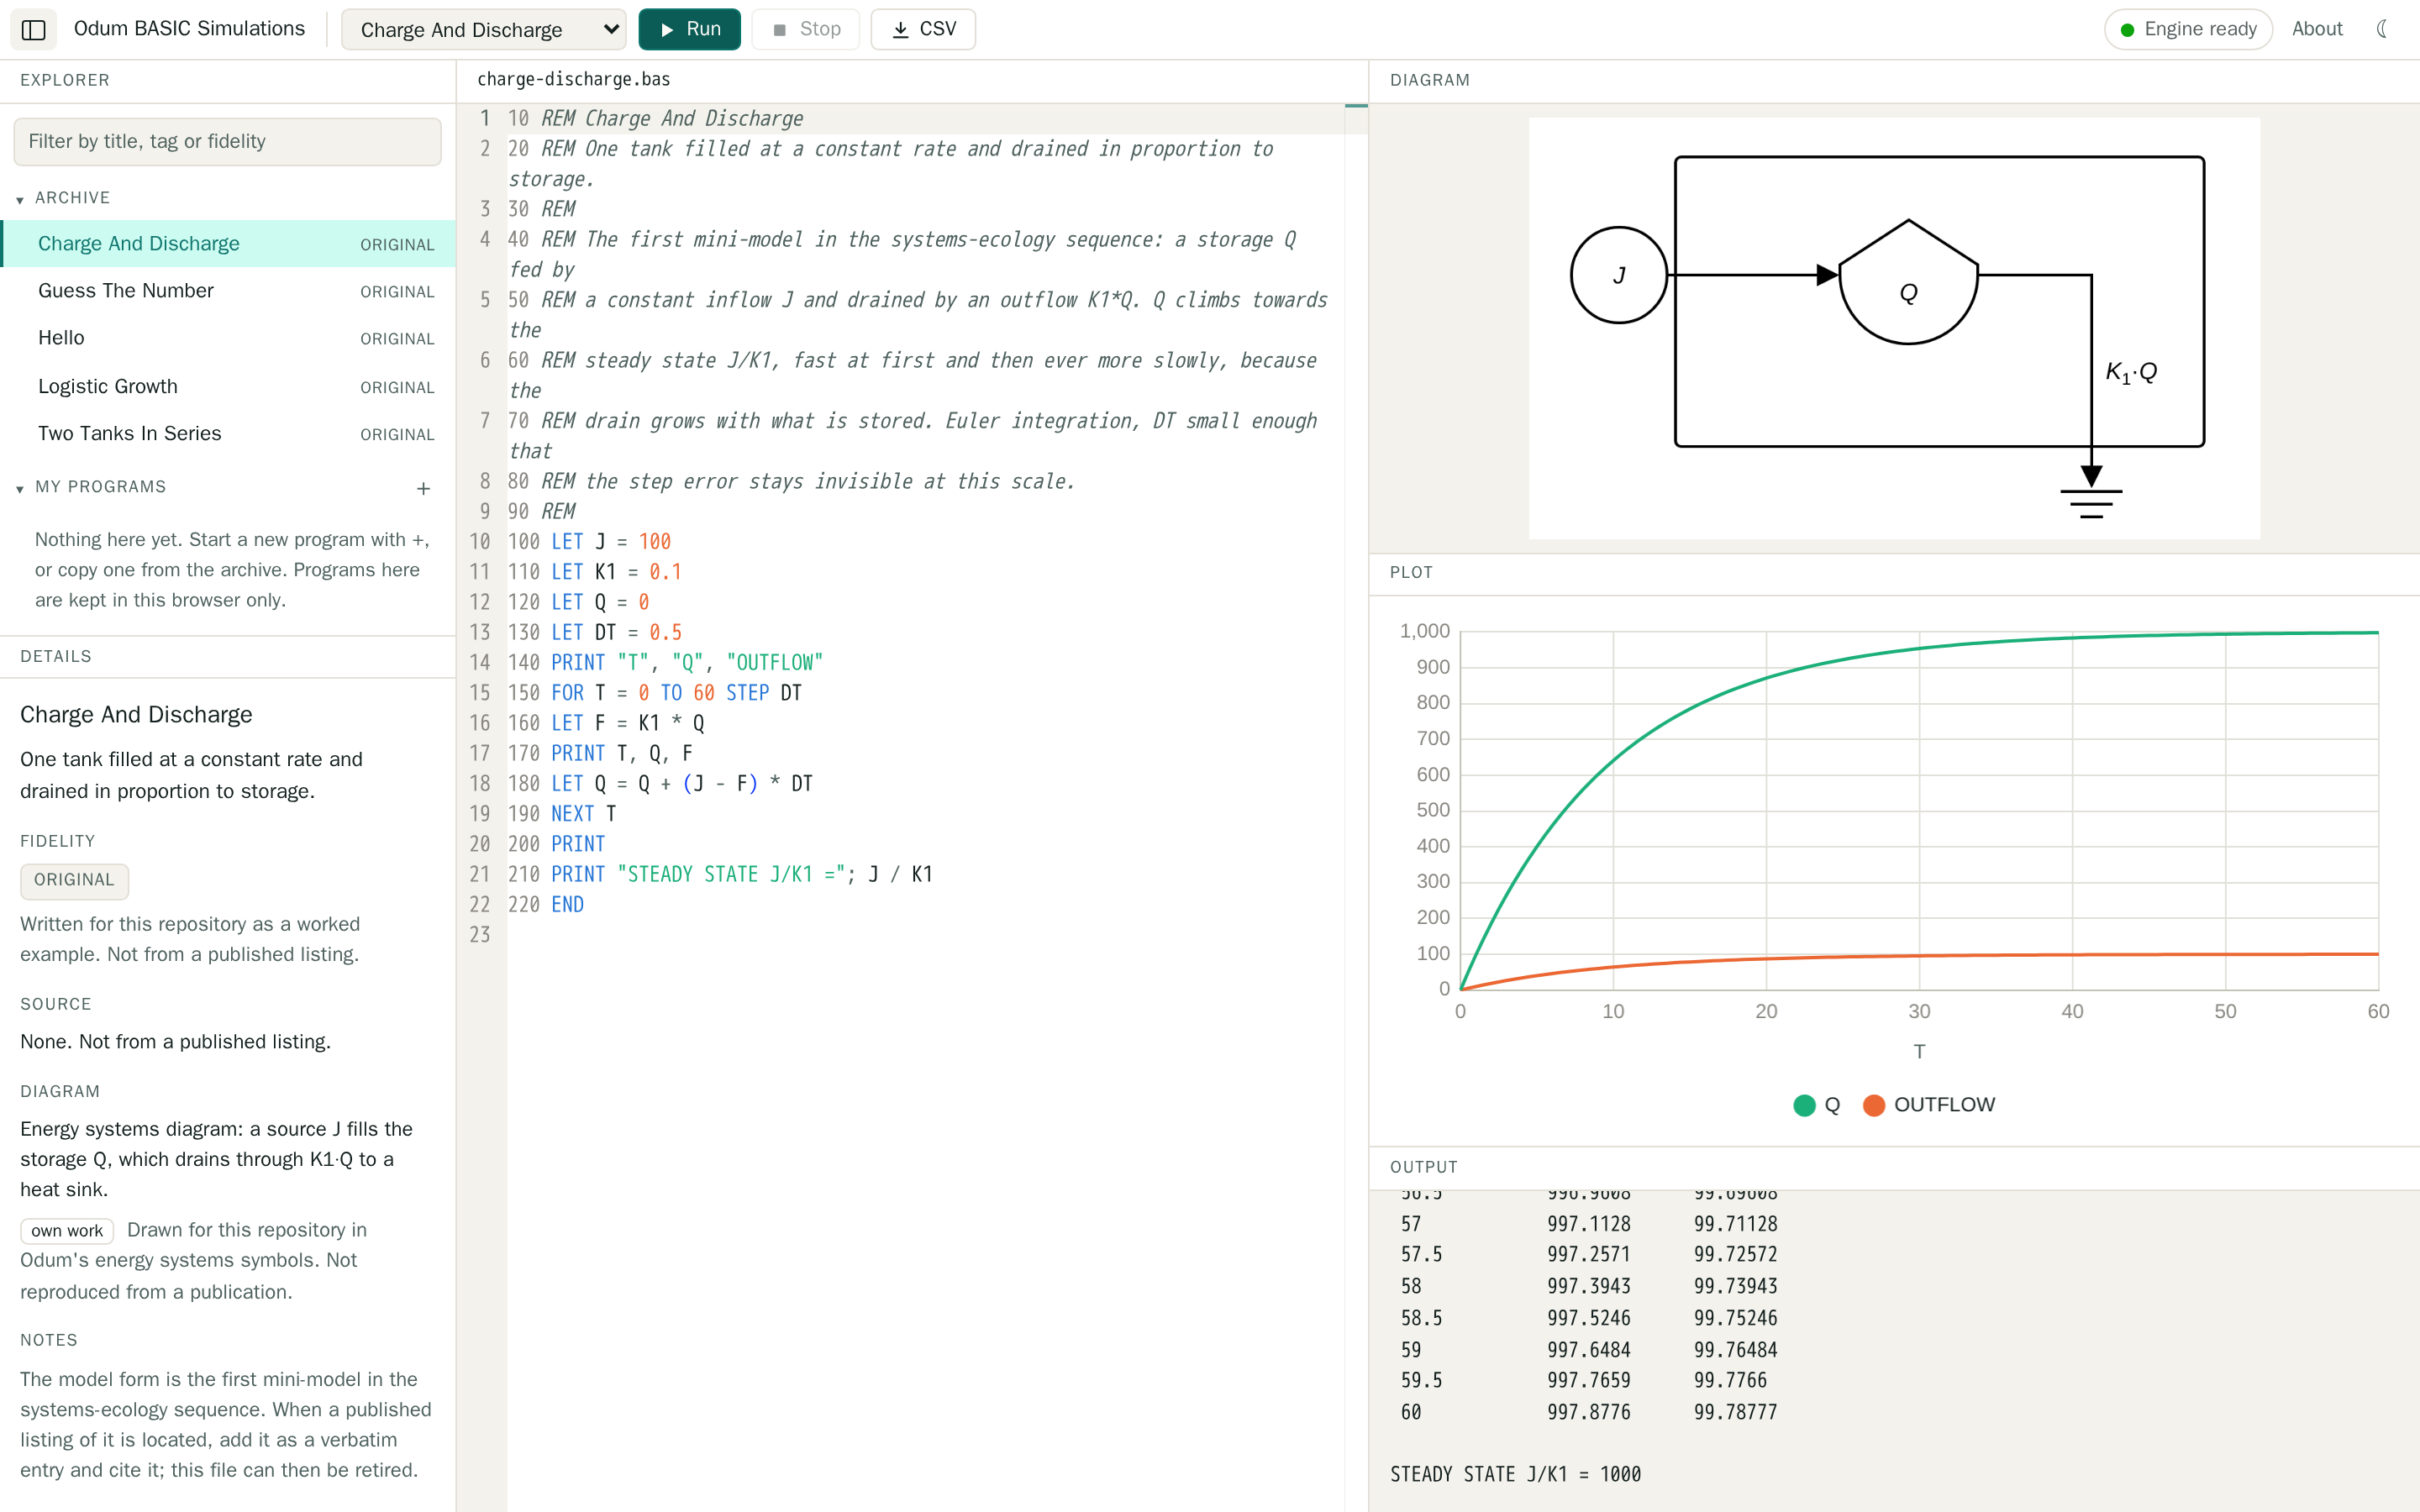
\includegraphics[width=0.8\linewidth]{workbench.png}
\caption{The browser-based workbench interface displaying the charge-and-discharge benchmark model following simulation execution, illustrating model navigation, source code editing, Energy Systems Language diagram rendering, tabular console output, and reconstructed phase trajectory plotting. The indicator at the upper right reports the state of the WebAssembly build of the C engine, which checks the listing in the editor as it is typed; it is a status of the checker alone, and simulation execution proceeds independently of it.}
\label{fig:workbench}
\end{figure*}

% RESOLVED(implementation/website): a paragraph on delivery now follows,
% covering instantiation, the in-editor checker, the shared-engine argument,
% the fail-open behaviour and the glue-free build.

\paragraph{Delivery to the browser} The WebAssembly module is fetched once per session and instantiated directly, both on the main thread, where the editor uses it, and inside the Web Worker that executes listings. Its diagnostics are emitted in the structure the editor's annotation interface already expects, and are therefore passed through without translation; the listing in the editor is re-checked as it is typed, so a reader modifying a historical program is shown immediately where it ceases to be valid BASIC for the selected dialect. The same compiled core backs the command-line tool's \texttt{check} subcommand, so the editor and the tool agree by construction rather than by two separately maintained implementations being kept in step --- an architectural property, not a testing outcome. The checker fails open: if the module cannot be retrieved, the editor continues to operate without annotations, on the reasoning that an editor which refuses to open because its checker is missing is worse than one which opens unchecked, and the interface indicator visible in Figure~\ref{fig:workbench} reports which of the two states obtains. The module is built without JavaScript glue code, as a standalone WebAssembly binary with no entry point; its only import is a memory-growth notification, because the validation path performs no input or output and therefore introduces no system-interface dependency. This is what keeps the committed artifact small enough to be reviewed and stable enough to be compared byte for byte against a rebuild.
Automated extraction of quantitative trajectories from legacy console output requires a systematic heuristic. Because historical simulation listings predate structured data-interchange formats, simulation results were sequentially emitted via formatted \texttt{PRINT} statements. The extraction engine scans the output stream for contiguous blocks of multi-column numeric data delimited by standard whitespace or tab tokens. The longest contiguous block sharing a constant field width is classified as the primary simulation table, with the initial column designated as the independent temporal variable. Column headers are automatically parsed from preceding non-numeric string labels. If the parsing heuristic fails to detect a consistent tabular structure, raw text streams remain fully accessible to the user, and resolved tables may be exported as standardized comma-separated values (CSV).

\begin{figure*}[t]
\centering
\begin{subfigure}[b]{0.42\linewidth}
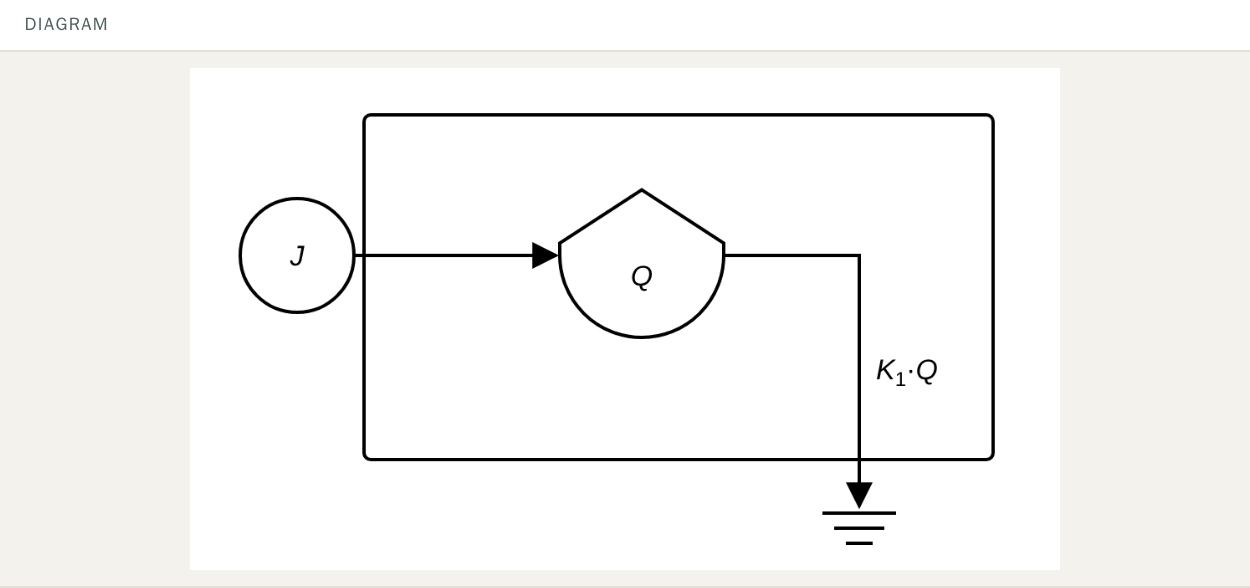
\includegraphics[width=\linewidth]{minimodel-diagram.png}
\caption{Energy Systems Language diagram.}
\end{subfigure}\hfill
\begin{subfigure}[b]{0.42\linewidth}
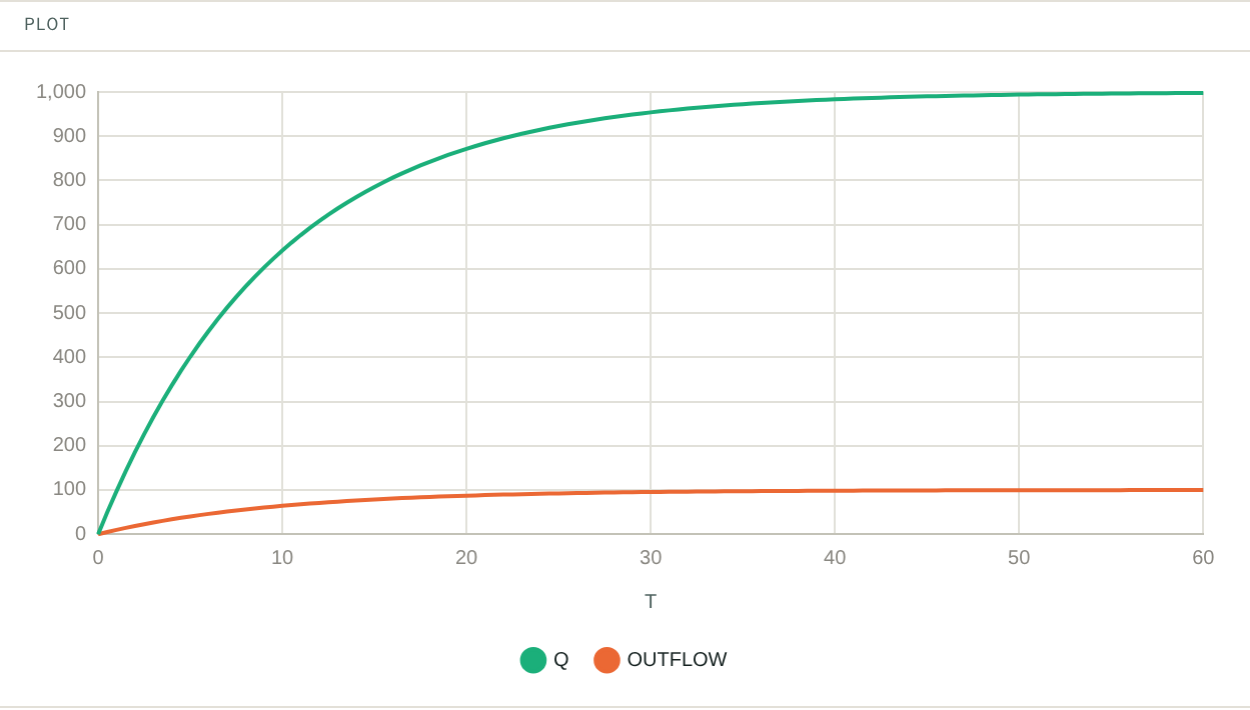
\includegraphics[width=\linewidth]{minimodel-plot.png}
\caption{Reconstructed simulation trajectory.}
\end{subfigure}
\caption{Dual representation of an ecological compartmental model within the archive: (a) visual Energy Systems Language diagram indicating forcing function $J$, storage $Q$, and donor-controlled outflow $K_1Q$; (b) corresponding dynamic trajectory recovered directly from the interpreted forward-Euler numerical integration output.}
\label{fig:minimodel}
\end{figure*}

The graphical workbench interface integrates these execution facilities into a unified analytical environment (Figure~\ref{fig:workbench}). The interface organizes models within an interactive catalog, displaying source listings alongside corresponding Energy Systems Language diagrams, recovered dynamic plots, and console execution logs (Figure~\ref{fig:minimodel}). Each program is addressable via persistent uniform resource identifiers, ensuring stable cross-referencing for scientific and educational applications.

The archival filesystem hierarchy enforces strict isolation between program definitions and relational metadata. Program modules are cataloged within a structured directory hierarchy containing legacy listings (\texttt{.bas}), standardized metadata specification files (\texttt{.json}), and accompanying raster diagrams. Published volumes containing multiple minimodels are aggregated into cohesive directory modules linked to master bibliographic records. Automated build pipelines enforce schema compliance across all entries, verifying that directory structures match declared citation keys and that modification diffs are preserved without altering verbatim source texts.

%% ----------------------------------------------------------------------------
\section{Ingestion workflows and provenance verification}
\label{sec:contributing}

To facilitate the expansion of the historical model corpus while maintaining archival integrity, the framework provides four ingestion pathways calibrated to varying technical requirements (Figure~\ref{fig:routes}, Table~\ref{tab:routes}).

\begin{table*}[t]
\centering\small
\begin{tabularx}{\linewidth}{@{}lXXX@{}}
\toprule
Ingestion pathway & User technical prerequisites & Automated validation & Human verification protocol \\
\midrule
Version-control pull request & Git version-control; JSON schema compliance & Static build validation; regression test harness & Code review; bibliographic verification \\
Structured issue form & Standard web access; repository account & Automated schema compilation and linting & Review of attached source documentation; approval \\
Interactive workbench & Client web browser & Dynamic schema validation; pre-filled issue staging & Visual comparison against primary literature scan \\
Automated transcription & Source scan or transcription prompt & Automated parsing; syntax check; test execution & Mandatory verification of numerical coefficients against original page \\
\bottomrule
\end{tabularx}
\caption{Summary of archival ingestion pathways, detailing operational prerequisites, automated validation routines, and human verification checkpoints.}
\label{tab:routes}
\end{table*}

The primary pathway utilizes formal version-control pull requests, enabling advanced contributors to supply complete program packages comprising source listings, diagram assets, and metadata files. Continuous integration pipelines validate all companion metadata files against the central JSON schema and run regression test suites prior to human code review.

\begin{figure*}[t]
\centering
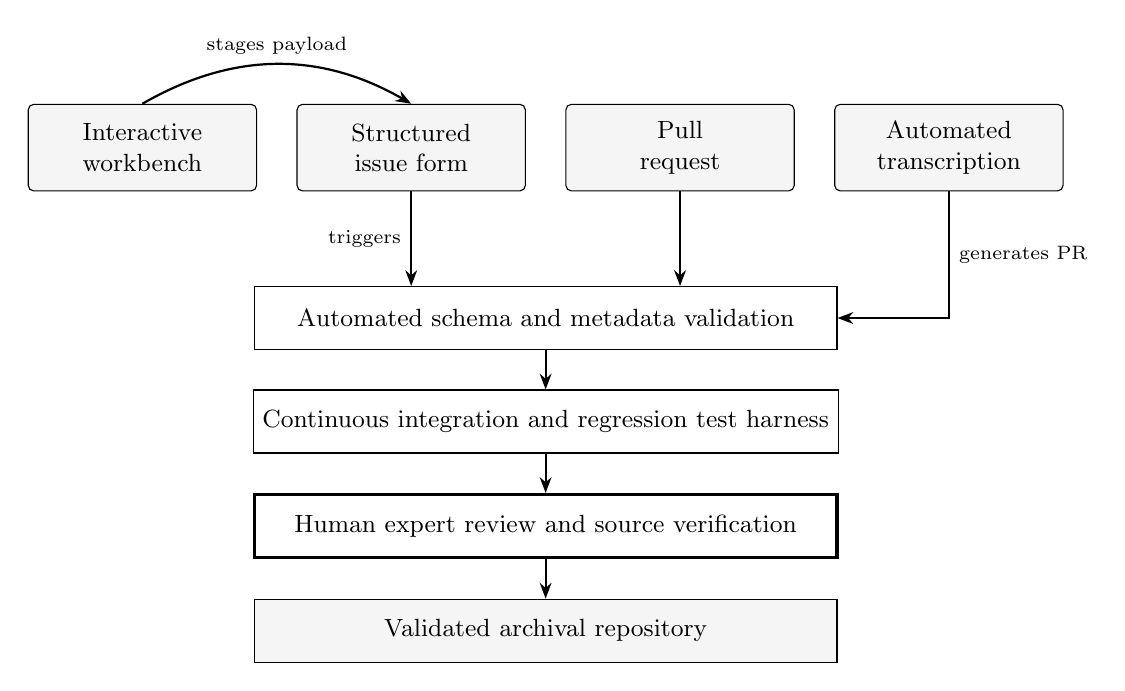
\begin{tikzpicture}[
  node distance=5mm and 5mm,
  every node/.style={font=\small, align=center},
  entry/.style={draw, rounded corners=2pt, minimum width=29mm, minimum height=11mm, fill=gray!8},
  stage/.style={draw, minimum width=74mm, minimum height=8mm},
  human/.style={stage, very thick},
  flow/.style={-{Stealth[length=2mm]}, thick},
]
\node[entry] (ws) {Interactive\\workbench};
\node[entry, right=of ws] (form) {Structured\\issue form};
\node[entry, right=of form] (pr) {Pull\\request};
\node[entry, right=of pr] (jules) {Automated\\transcription};
\node[stage, below=12mm of $(form.south)!0.5!(pr.south)$] (val) {Automated schema and metadata validation};
\node[stage, below=of val] (ci) {Continuous integration and regression test harness};
\node[human, below=of ci] (rev) {Human expert review and source verification};
\node[stage, below=of rev, fill=gray!8] (arc) {Validated archival repository};
\draw[flow] (ws.north) to[bend left=30] node[above, font=\scriptsize] {stages payload} (form.north);
\draw[flow] (form.south) -- node[left, font=\scriptsize] {triggers} (val.north -| form.south);
\draw[flow] (pr.south) -- (val.north -| pr.south);
\draw[flow] (jules.south) |- node[pos=0.25, right, font=\scriptsize] {generates PR} (val.east);
\draw[flow] (val) -- (ci);
\draw[flow] (ci) -- (rev);
\draw[flow] (rev) -- (arc);
\end{tikzpicture}
\caption{Architectural schema of the ingestion and verification pipeline, illustrating automated validation, continuous integration testing, and human-in-the-loop review criteria across all four contribution pathways.}
\label{fig:routes}
\end{figure*}

To lower technical barriers for domain specialists in ecology who may not utilize distributed version-control tools, a secondary pathway leverages structured issue forms. Contributors submit program listings, bibliographic data, and visual scans through standardized web form fields. An automated repository workflow parses the submitted issue payload, compiles the corresponding metadata files, and triggers the central validation suite. Diagnostic feedback is returned automatically if required parameters are missing or malformed. Once validation succeeds, an automated pull request is generated, preserving contributor attribution while staging the submission for human verification.

The third pathway operates within the interactive workbench. Contributors draft, execute, and annotate models within a private local browser workspace. The interface performs continuous schema validation during editing. Upon completion, the workspace compiles the metadata and redirects the user to the structured submission form with all fields pre-populated, preventing manual formatting errors.

A fourth ingestion pathway accommodates automated transcription from digitized document scans. Because automated optical character recognition can introduce subtle numerical inaccuracies in mathematical coefficients without generating syntax errors, this pathway is constrained by strict oversight protocols: automated transcription agents are restricted to clerical code extraction, and repository maintainers are required to perform line-by-line manual verification against primary source scans before merging.

Diagram preservation requires distinct intellectual property governance. The archive records formal rights statements for every visual asset, cataloging the reproduction basis (e.g., author-created, public domain, authorized permission, or fair-use scholarship review) alongside precise page and figure attributions. Binary diagram formats are restricted to static raster representations (PNG, JPEG) to prevent security risks associated with executable script contexts in vector formats.

%% ----------------------------------------------------------------------------
\section{AI-assisted implementation and verification methodology}
\label{sec:llm}

In accordance with institutional guidelines governing the disclosure of artificial intelligence technologies in scientific research \citep{elsevierAI}, this section details the formal protocols, toolchains, and test-driven validation criteria employed during the development of the execution runtime.

The runtime architecture, parsing modules, and metadata validation suites were implemented utilizing Claude Code \citep{claudeCode}, an agentic development tool operating with the Claude Opus~5 language model, under continuous human direction. The methodological division of responsibility maintained human ownership over system architecture, mathematical formulations, dialect precedence rules, and intellectual property governance, while leveraging the language model for rapid code drafting, test construction, and documentation synthesis. Direct automated modifications to production branches were prohibited: all generated code was committed to isolated task branches and required successful passage through automated regression harnesses and human code review prior to integration.

To mitigate known failure modes associated with automated code generation—including hallucinated language features, silent numerical edge-case failures, and architectural regression—the development lifecycle enforced six procedural controls:
\begin{enumerate}
\item \textbf{Specification-first test-driven implementation:} Explicit unit assertions and behavioral expectations were defined prior to the synthesis of functional runtime modules.
\item \textbf{Dual-layer integration testing:} Automated test pipelines executed test suites across both raw development sources and compiled, bundled deployment packages to detect toolchain-induced discrepancies.
\item \textbf{Isolated development worktrees:} Concurrent programming tasks were executed within segregated git worktrees, preventing cross-task state contamination.
\item \textbf{Machine-checkable visual regression testing:} Automated browser automation harnesses captured rendered interface states against pinned golden reference images, verifying that visual outputs, plotting canvases, and layout structures remained invariant across modifications.
% RESOLVED(llm/controls): the attestation is now control 6, with the
% distinction drawn between checking that code satisfies a test and checking
% that published results can still be regenerated.
\item \textbf{Granular commit auditing:} Machine-assisted commits incorporated standardized co-author trailers, providing an immutable audit trail of automated contributions within the repository history.
\item \textbf{Regeneration attestation:} Every result underlying the comparisons reported in Section~\ref{sec:validation} is regenerated from source within digest-pinned container images and compared against a recorded SHA-256 digest, and the committed WebAssembly artifact is rebuilt and rejected if a single byte differs from the version in the repository. Both checks execute on every proposed change. This control differs in kind from the preceding five: those establish that the code satisfies an assertion an author wrote, whereas this establishes that the numerical and graphical results published in this paper can still be produced from the archived source --- which is the property the paper is itself about, and the one most vulnerable to silent decay.
\end{enumerate}

% RESOLVED(llm/efficacy): the INPUT-as-DIM defect is now reported in the text
% below, with the sample-of-one assertion named as the cause and the closing
% claim qualified accordingly. "Two releases" was verified against the history:
% the defect was live from the merge that shipped the WebAssembly checker until
% the merge that implemented INPUT, spanning two deployments.
The efficacy of these validation controls was evaluated empirically against subtle implementation errors encountered during runtime construction. For example, integration testing identified an unhandled temporal index offset in a synthetic two-tank benchmark listing, wherein an inflow termination condition was evaluated subsequent to state integration, shifting effective cutoff timing by two integration intervals. Similarly, during the implementation of graphics coordinate transformations, regression testing revealed discrepancies in midpoint coordinate rounding between modern floating-point conversions and legacy PC rasterization routines. In each instance, automated test failures or explicit source discrepancies halted integration, necessitating human architectural intervention.

Reporting only the defects the controls intercepted would overstate them, and one failure reached the deployed application. The C engine selected its handler for a statement by performing arithmetic on the keyword enumeration. The \texttt{INPUT} keyword does not adjoin \texttt{DIM} in that enumeration, so the subtraction underflowed as an unsigned index, passed the subsequent bounds test, and selected entry zero: every \texttt{INPUT} statement was consequently parsed as a \texttt{DIM}. The misparse validated cleanly wherever the statement resembled a declaration, which the bare form \texttt{INPUT G} does, and nothing failed until the prompted form used by an archived listing was checked, at which point the editor reported a published listing as syntactically broken. Two deployments shipped in that state. The control that should have caught this was present: a test asserting that every published listing must pass the checker. The assertion was wrong rather than absent --- it checked a single listing while being written as a guarantee about a corpus. The remedy was to check the entire corpus, and the regression guard was confirmed to fail against the previously committed artifact before it was permitted to pass.

This failure is methodologically more informative than the successes above, and it qualifies the conclusion. These observations reinforce established findings in empirical software engineering: while automated language models demonstrate high proficiency in generating localized algorithms to formal specifications \citep{chen2021}, their deployment in complex systems requires formal testing harnesses and human domain expertise to ensure scientific integrity \citep{jimenez2024}. The qualification is that a harness bounds what a model can silently get wrong only to the extent that its assertions state what their author believes they state. A generated test that names the right property and then verifies a sample of one reads, in review, exactly like a test that verifies the property.

\begin{table}[tb]
\centering\small
\begin{tabularx}{\linewidth}{@{}Xr@{}}
\toprule
Architectural component & Metric count \\
\midrule
Pull requests integrated & 36 \\
Non-merge development commits & 49 \\
C engine source and header lines (executing implementation) & 2{,}664 \\
\quad committed WebAssembly artifact & 68\,KB \\
TypeScript source lines (application, archive and utilities) & 6{,}898 \\
\quad of which the reference BASIC interpreter & 1{,}024 \\
Styling and interface markup lines & 1{,}953 \\
Automated test suite volume (lines of test code) & 4{,}807 \\
\quad of which C engine test suites & 872 \\
Unit test assertions & 236 \\
End-to-end integration test assertions (development and release builds) & 113 \\
Visual regression golden assertions & 4 \\
Attested regeneration results & 33 \\
\bottomrule
\end{tabularx}
% RESOLVED(llm/table): regenerated at 76fa9a9, not copied from the marker --
% which was itself measured at 56a43e8 and had gone stale again. The C engine
% now has its own rows. TypeScript source is src/ excluding *.test.ts; test
% volume is src/**/*.test.ts plus e2e/ plus engine/tests/. Regenerate again
% before submission; the commands are in the pull request that added this.
\caption{Quantitative structural metrics of the reconstructed execution framework and validation test harness, derived from the version-controlled release repository.}
\label{tab:llm}
\end{table}

% RESOLVED(llm/ratio): recomputed from the regenerated table, with the
% denominator stated rather than left implicit (the original 37% excluded
% styling and markup, which was not said).
The resulting codebase (Table~\ref{tab:llm}) maintains a substantial ratio of verification logic to runtime logic: automated test harnesses comprise 4{,}807 lines against 9{,}562 lines of executable source across both implementations, or approximately 33\% of the combined total, excluding styling and interface markup. This ratio understates the verification effort, because it counts only test code and not the attestation records, the pinned golden images, or the second implementation itself, whose purpose is verification rather than delivery. This infrastructure provides the empirical basis for trusting a computational engine constructed through AI-assisted development methodologies --- subject to the qualification established above, that an assertion binds only what it actually states.

%% ----------------------------------------------------------------------------
\section{Validation and numerical analysis}
\label{sec:validation}

% RESOLVED(validation/tiers): promoted to four tiers, with independent
% reimplementation given its own subsection rather than folded into the
% emulator comparison. They answer different questions: the emulator asks
% whether we agree with a period-faithful reference, the second implementation
% asks whether agreement is a property of the language core or an artefact of
% one program that happens to compute it.
Evaluating the reliability of the reconstructed runtime requires four complementary lines of empirical evidence: comparative verification against analytical solutions of canonical ecological systems, cross-platform validation against emulated historical interpreters, agreement between two independently written implementations of the language core, and concordance testing against historical printed outputs. The third of these is not a variant of the second. An emulator constrains systematic error only to the degree that it shares no ancestry with the runtime under test, which is an assumption about provenance; a second implementation, written separately from the same specification and computing at a different precision, tests that assumption directly.

\subsection{Analytical verification on canonical compartmental models}

The initial validation tier evaluates the numerical execution engine against three canonical compartmental models characterized by closed-form analytical solutions:
\begin{enumerate}
\item \textbf{Linear charge-and-discharge storage:} A single-state reservoir governed by constant input flux $J$ and linear, donor-controlled drainage $K_1Q$:
\begin{equation}
\begin{gathered}
\frac{\mathrm{d}Q}{\mathrm{d}t} = J - K_1Q, \\
Q(t) = \frac{J}{K_1}\left(1 - e^{-K_1t}\right).
\end{gathered}
\end{equation}
\item \textbf{Logistic growth resource model:} A self-limiting biological population exhibiting density-dependent saturation:
\begin{equation}
\begin{gathered}
\frac{\mathrm{d}Q}{\mathrm{d}t} = K_1Q(S_T - Q) - K_2Q, \\
Q(t) = \frac{C}{1 + \left(\frac{C - Q_0}{Q_0}\right)e^{-rt}},
\end{gathered}
\end{equation}
where intrinsic growth rate $r = K_1S_T - K_2$ and carrying capacity $C = S_T - K_2/K_1$.
\item \textbf{Two-stage linear cascade with step forcing:} A coupled linear system ($\mathrm{d}Q_1/\mathrm{d}t = J - K_1Q_1$, $\mathrm{d}Q_2/\mathrm{d}t = K_1Q_1 - K_2Q_2$) subject to a piecewise step-down in forcing $J$ at time $t_c$, yielding exponential decay phases across both state variables.
\end{enumerate}

Each model listing executes an explicit forward-Euler integration recurrence over discrete time increments $\Delta t$. In automated validation tests, the output of the C engine --- the implementation the site executes --- was compared across every time step against an independent recurrence evaluation performed in identical operational sequence and at identical precision, as well as against the analytical solution (Table~\ref{tab:validation}).

\begin{table*}[t]
\centering\small\setlength{\tabcolsep}{4pt}
\begin{tabular}{@{}lrrcc@{}}
\toprule
& & & \multicolumn{2}{c@{}}{Maximum relative error} \\
\cmidrule(l){4-5}
Benchmark model & $\Delta t$ & Output rows & Engine vs.\ recurrence & Recurrence vs.\ analytical \\
\midrule
Linear charge-and-discharge & 0.50 & 121 & $\le 5\times10^{-7}$ & 0.94\% \\
Logistic growth & 0.50 & 401 & $\le 5\times10^{-7}$ & 7.41\% \\
Coupled linear cascade ($t_c = 40.5$) & 0.25 & 321 & $\le 5\times10^{-7}$ & 0.70\% \\
Coupled linear cascade ($t_c = 40.0$, nominal) & 0.25 & 321 & $\le 5\times10^{-7}$ & 7.27\% \\
\bottomrule
\end{tabular}
\caption{Numerical validation of the C engine across canonical compartmental models. Discrepancies between engine output and independent single-precision forward-Euler recurrences fall strictly within the rounding of the console display routine, which gives a single seven significant digits; expressed as a fraction of the value, its worst case is $5\times10^{-7}$. On every row of every listing the difference is within half a unit in that row's own last printed digit, so the two computations agree exactly and only the display separates them. Discrepancies between recurrence sequences and exact analytical solutions reflect standard discretization truncation errors inherent to first-order Euler integration, and are unchanged by the move to single precision.}
\label{tab:validation}
\end{table*}

% RESOLVED(validation/precision): execution moved to the C engine, and the
% reference recurrence moved to single precision with it (Math.fround on every
% literal and after every operation, in the listing's own order). The threshold
% stayed where it was, as predicted. Measured by validation.test.ts:
%
%   charge-discharge    0.996 half-quanta   2.4e-7 of the value
%   logistic-growth     1.000 half-quanta   3.9e-7 of the value
%   two-tank (40.5)     0.999 half-quanta   4.5e-7 of the value
%   two-tank (40.0)     0.999 half-quanta   4.5e-7 of the value
%
% "Half-quanta" is the difference as a multiple of half a unit in the last digit
% PRINT showed for that value; at most 1 means the printed value IS the
% recurrence rounded to what PRINT shows. The test fails by 3x to 24x if the
% Math.fround is removed, so the tolerance is load-bearing rather than
% decorative. The "Recurrence vs. analytical" column did not move: single
% precision does not touch first-order truncation error at these step sizes.
Across all evaluated rows, the engine output coincided with the independent single-precision recurrence to within the rounding of the console display routine, which gives a single seven significant digits ($\le 5\times10^{-7}$ of the value, and within half a unit of each row's own last printed digit). The remaining deviations between the numerical trajectories and the analytical benchmarks represent standard numerical truncation error characteristic of first-order forward-Euler integration: below 1\% for the linear models, and 7.41\% for the logistic model, whose effective parameter product ($r\Delta t = 0.19$) introduces greater discretization error. In the coupled cascade model, evaluating the nominal listing exposed an execution timing offset: because the conditional termination statement (\texttt{IF T > 40 THEN LET J = 0}) was sequenced following state updates, the effective inflow cut occurred at $t = 40.5$ rather than $t = 40.0$, elevating analytical error from 0.70\% to 7.27\%. Preserving such anomalies within the archive illustrates the necessity of executing listings directly rather than relying on textual descriptions.

\subsection{Cross-platform validation against emulated historical runtimes}

The second validation tier examines the numerical and graphical correspondence between the reconstructed runtime and an emulated historical execution environment. The evaluation examined a published systems ecology listing modeling macroeconomic-resource interactions over 640 forward-Euler integration steps with state-dependent threshold switching \citep[Table~3]{odum1989}. The model was executed simultaneously within the reconstructed web runtime and within PC-BASIC \citep{pcbasic}, an open-source emulator that replicates GW-BASIC architecture and Microsoft Binary Format floating-point representations.

\begin{table*}[t]
\centering\small
\resizebox{\linewidth}{!}{\oracleTable}
\caption{Comparative numerical evaluation of Odum (1989, Table~3) across 640 forward-Euler integration steps executed within the reconstructed interpreter (R1, R4a, R4b) and the PC-BASIC reference emulator (R2, R3, R3d). The maximum relative difference reflects deviations across all state variables. Plotted pixel agreement indicates coordinate identity across all 2,560 trajectory points. Bit-identical steps quantify exact binary floating-point concordance with the single-precision emulator reference.}
\label{tab:oracle}
\end{table*}

Because the reconstructed interpreter computes using IEEE-754 double-precision arithmetic whereas GW-BASIC utilized MBF single-precision by default, divergence between modern and historical trajectories could arise from numerical precision differences. However, as documented in Table~\ref{tab:oracle}, precision divergence does not alter macro-scale model behavior. The maximum relative difference between modern double-precision execution and legacy single-precision emulation remained bounded at $4.0\times10^{-5}$, primarily localized in a state variable constrained to a minimum floor of 0.0001. Across all 2,560 plotted trajectory coordinates, screen-space displacement did not exceed $6.8\times10^{-5}$ pixels, resulting in 100\% visual pixel concordance across the rendered trajectories. Furthermore, dynamic threshold switching (\texttt{IF D > 30 THEN IV = 0}) occurred identically at step 263 ($t = 131.5$) across all execution environments. When double-precision variables were emulated within the reference platform (Run R3d), numerical concordance reached $3.7\times10^{-13}$, verifying that the statement semantics of the interpreter introduce no algorithmic distortion.

\begin{figure*}[t]
\centering
\begin{subfigure}{0.42\linewidth}

\includegraphics[width=\linewidth]{r2.png}
\caption{Reference emulator screen output}
\end{subfigure}\hfill
\begin{subfigure}{0.42\linewidth}

\includegraphics[width=\linewidth]{r1-diff.png}
\caption{Reconstructed display difference map}
\end{subfigure}
\caption{Comparative rasterization analysis of Odum (1989, Table~3) in \texttt{SCREEN 1} mode (320$\times$200 pixels). (a) Emulated video buffer output generated by PC-BASIC. (b) Reconstructed canvas output, with 111 differing pixels highlighted in white. The discrepancy was traced to divergent midpoint rounding conventions between the emulator and primary GW-BASIC interpreter source code.}
\label{fig:oracle}
\end{figure*}

Cross-platform raster comparison revealed an informative implementation divergence. Comparing the emulated video memory of PC-BASIC with the reconstructed canvas buffer identified an apparent spatial mismatch across 111 of 64,000 pixels (Figure~\ref{fig:oracle}). Emulating single-precision arithmetic did not alter this mismatch, indicating that the variation arose from coordinate discretization rather than numerical drift. Analysis revealed that the temporal increment of 0.5 units mapped alternate integration steps exactly to half-pixel coordinates. PC-BASIC's rasterization routine rounded half-integers to the nearest even integer (round-half-to-even), whereas the reconstructed runtime rounded half-integers away from zero. 

Applying the hierarchical evidentiary criteria defined in Section~\ref{sec:design}, this conflict was arbitrated through examination of primary source artifacts. Within the released assembly source code of GW-BASIC \citep{gwbasic}, graphics coordinate conversion calls the internal routine shared by the integer conversion function \texttt{CINT}, which implements symmetric round-half-away-from-zero rounding. Consequently, the reconstructed runtime's coordinate mapping conformed to the historical hardware implementation, whereas the emulator exhibited an undocumented internal deviation. Resolving this discrepancy demonstrates the value of multi-engine comparative validation in computational software archaeology.

\subsection{Independent reimplementation of the language core}

A reconstructed runtime that recovers a historical trajectory establishes that the trajectory is recoverable; it does not establish that the recovery is independent of the particular program performing it. A systematic error in the interpreter would be reproduced faithfully by every run of that interpreter, and agreement with an emulator constrains this only insofar as the two share no common ancestry. To separate these, the language core was implemented a second time, in C, and compiled both to a native command-line executable and to WebAssembly for in-browser use. The comparison reported here was performed when the TypeScript interpreter was still the executing implementation and the C engine the newcomer; the roles have since exchanged, and the engine is now the runtime described in Section~\ref{sec:implementation}, with the interpreter retained as the reference. The comparison is unaffected by which of the two the site invokes, and is repeated on every proposed change. The C implementation computes in single precision by type rather than in double precision, and enforces its arithmetic contract at compile time: intermediate results may not be evaluated at wider precision (\texttt{FLT\_EVAL\_METHOD} equal to zero), and floating-point contraction is disabled, so that a fused multiply-add cannot round once where the original rounded twice.

Executing the same listing through this implementation (Run R5) and rasterizing its output through the display routine shared with the primary interpreter yields a screen differing from that interpreter's in \oracleEnginesDiffering{} of \oracleScreenPixels{} pixels, and differing from the PC-BASIC reference in \oracleEngineScreenDiffering{}---the identical disparity exhibited by the primary interpreter, and attributable to the same midpoint rounding convention analyzed above. Rounding to single precision after every operation within the TypeScript interpreter likewise alters \oraclePrecisionsDiffering{} pixels. Two independently written implementations, in different languages and at different arithmetic precisions, therefore reconstruct the published figure identically, which localizes the residual disparity in the rasterization convention rather than in either interpreter or in the choice of numeric format. This comparison is regenerated and verified on every proposed change to the repository, so the agreement is a maintained property rather than a single historical measurement.

\subsection{Concordance with historical printed output}

The fourth tier of validation---direct automated verification against original printed output tables and published figure scans---represents an ongoing empirical objective that requires progressive expansion of the verified listing corpus.

%% ----------------------------------------------------------------------------
\section{Discussion}
\label{sec:discussion}

The restoration of execution fidelity to historical ecological models provides a rigorous computational foundation for evaluating early systems ecology literature. In computational science, publishing source code listings without an active runtime provides incomplete reproducibility; when software environments decay, scientific claims become unfalsifiable. By reconstructing an open, web-accessible execution environment, historical simulation listings are transformed from static typographical records into active computational experiments that can be verified, audited, and extended.

This capability facilitates several investigative avenues in systems ecology:
\begin{itemize}
\item \textbf{Direct verification of published trajectories:} Researchers can independently evaluate whether published forward-Euler algorithms faithfully reproduce the phase behaviors and transient responses depicted in printed figures. Discrepancies between printed narratives and algorithmic behavior—such as the step-forcing timing offset observed in Section~\ref{sec:validation}—can be identified and documented rather than obscured by modern re-implementations.
\item \textbf{Pedagogical accessibility:} Students and researchers can interact directly with historical models within a standardized browser environment, exploring parameter sensitivities and dynamic properties without requiring specialized emulation toolchains or obsolete hardware.
\item \textbf{Dual-formalism consistency testing:} In Odum's systems ecology, models were simultaneously specified as visual Energy Systems Language diagrams and as executable differential equations. Because visual and mathematical formalisms can drift apart during publication, a verified execution archive provides an essential empirical benchmark for evaluating automated diagram-to-model compilation environments \citep{energese,gssk}.
\end{itemize}

From a software preservation perspective, this investigation highlights a fundamental methodological distinction between software evolution analysis and runtime reconstruction. Standard software archaeology interrogates dynamic repositories to trace code modifications over time \citep{huntThomas2002,robles2005,spinellis2021}. For historical scientific listings, the preservation target is not an evolving code repository but an immutable printed artifact whose operational context has dissolved. Preserving such models requires an evidential approach to runtime reconstruction, governed by strict source hierarchies and transparent provenance tracking.

The introduction of formal fidelity classifications (Table~\ref{tab:fidelity}) addresses an important omission in contemporary research software preservation frameworks. While the FAIR4RS guidelines \citep{barker2022} define essential criteria for discoverability and licensing, they presume that preserved code represents an authentic primary artifact. In historical computational recovery, distinguishing between verbatim transcriptions, errata-corrected listings, and modern algorithmic adaptations is paramount. Standardizing fidelity metadata ensures that scientific users can clearly differentiate between historical modeling artifacts and contemporary enhancements.

Similarly, establishing explicit rights metadata for accompanying visual diagrams provides a structured framework for managing intellectual property in scientific archives. While computational algorithms expressing scientific equations occupy distinct legal copyright parameters, visual diagrams require explicit attribution and rights declarations. Incorporating per-figure rights metadata balances open scientific dissemination with rigorous copyright compliance.

\subsection{Limitations and future research}

Several technical boundaries bound the current implementation:
\begin{enumerate}
\item \textbf{Language dialect coverage:} The current interpreter core supports the standard procedural and graphical statements characteristic of Odum's minimodels, but omits advanced structured control constructs (\texttt{WHILE/WEND}, \texttt{SELECT CASE}) and specialized string-formatting commands (\texttt{PRINT USING}, \texttt{LOCATE}). Expanding dialect coverage is required to accommodate larger simulation listings.
% RESOLVED(limitations): the marker this replaces listed the C engine's
% missing INPUT and PRINT text as the limitation. Both were implemented
% (#34, #35), execution moved across (#37, #38), and the arithmetic moved to
% single precision with it, which is now reported in sec:validation rather than
% projected as a consequence. The genuine remaining divergence between the two
% implementations is narrower and is stated below.
\item \textbf{Divergence between the two implementations:} The reference interpreter and the executing engine are not interchangeable in every detail. A \texttt{PSET} statement that omits its color argument resolves to the highest color of the current mode in the reference implementation and to the most recently selected color in the engine; no listing in the archive depends on the difference, because each names its color explicitly, but the divergence is recorded rather than resolved by fiat. More generally, the two implementations are verified to agree on the archive's listings and on the compared published listing, which is evidence about that corpus and not a proof of equivalence.
\item \textbf{Empirical corpus expansion:} The present study validates the runtime architecture primarily against canonical benchmark models and selected historical listings. Transcribing, validating, and cataloging the extensive corpus of models distributed across Odum's foundational texts \citep{odum1983,odumMinimodels,odumOdum2000} constitutes an ongoing archival effort.
\item \textbf{Automated raster validation:} While graphical outputs can be rendered and compared at the pixel level, automated validation against historical scanned diagrams requires the development of robust visual comparison metrics that account for paper aging, print distortions, and scanner artifacts.
\end{enumerate}

%% ----------------------------------------------------------------------------
\section{Conclusions}
\label{sec:conclusions}

The computational preservation of historical scientific literature requires restoring the execution environments upon which computational claims depend. H.T. Odum and his collaborators documented systems ecology through fully disclosed, executable BASIC programs, yet the obsolescence of vintage computing environments rendered these models historically inaccessible.

% RESOLVED(conclusions): revised in step with the abstract; the
% independent-reimplementation result is now the closing claim.
Odum BASIC Simulations addresses this challenge by providing an open-source, web-standard execution runtime and archival repository that executes historical simulation listings without textual modernization. By enforcing machine-checked provenance schemas, formal fidelity taxonomies, and hierarchical evidence arbitration, the framework restores computational repeatability to historical systems ecology models. Numerical evaluations demonstrate that the reconstructed runtime achieves exact arithmetic concordance with legacy forward-Euler recurrences, differing from them by no more than the rounding of its own printed output, and resolves subtle historical rasterization semantics through primary interpreter source analysis. The strongest evidence the work provides, however, is not agreement with a reference but agreement between independents: two implementations of the language core, written separately in two languages and computing at two arithmetic precisions, reconstruct the published figure as the same screen. That localizes the sole remaining discrepancy in a documented rasterization convention rather than in either implementation, and because the comparison is regenerated and verified on every change to the repository, it is a maintained property of the archive rather than a measurement taken once. This computational framework bridges the gap between historical scientific literature and modern reproducibility standards, ensuring that foundational ecological models remain accessible for inspection, validation, and scientific inquiry.

%% ----------------------------------------------------------------------------
\section*{Software and data availability}

\begin{description}
\item[Software Title] Odum BASIC Simulations
\item[Developer] S. Maud
\item[Source Code Repository] \url{https://github.com/energese-project/Odum-basic-simulations}
\item[Operational Web Application] \url{https://energese-project.github.io/Odum-basic-simulations/}
\item[Software License] MIT License
\item[Archival Identifier] Zenodo DOI: [DOI to mint]
% RESOLVED(availability): all three corrected. The Node version is read from
% .node-version (26 at the time of writing); check it again before submission.
\item[Execution Requirements] Using the archive requires only a web browser supporting ECMAScript 2022; nothing below applies to a reader who wishes to run the published listings. Building and testing the site requires Node.js at the version pinned in the repository (26 at the time of writing), the unit suite executing TypeScript sources directly, or an equivalent OCI-compliant container environment. Rebuilding the WebAssembly module additionally requires an Emscripten toolchain, supplied as a digest-pinned container image; it is not needed to build or deploy the site, because the compiled artifact is committed to the repository. Reproducing the emulator comparison requires a container runtime in order to execute PC-BASIC.
% RESOLVED(availability/data): the two artefact-provenance commands are now
% named alongside the attestation.
\item[Data and Test Corpora] All simulation models, metadata sidecar specifications, visual regression baselines, and cross-runtime verification scripts are maintained within the open-access project repository. Reference comparison datasets generated via \texttt{make attest} are archived within the \texttt{validation/oracle/} directory, each recorded against a SHA-256 digest that the same command reverifies. Two further commands establish the provenance of the committed binary artifact: \texttt{make wasm} rebuilds the WebAssembly module within the pinned toolchain image, and \texttt{engine/build-wasm.sh -{}-check} rebuilds it and fails if the committed bytes no longer follow from the source. Both execute in continuous integration on every proposed change.
\end{description}

\section*{CRediT authorship contribution statement}
\textbf{S. Maud:} Conceptualization, Methodology, Software, Formal analysis, Validation, Investigation, Data curation, Writing -- original draft, Writing -- review \& editing.

\section*{Declaration of competing interest}
The author declares that there are no known competing financial interests or personal relationships that could have appeared to influence the work reported in this paper.

\section*{Declaration of generative AI and AI-assisted technologies in the manuscript preparation process}
During the preparation of this manuscript, the author utilized Claude Code (Anthropic; model Claude Opus~5) to assist in drafting initial section outlines, generating descriptive summaries of software metrics, and executing automated regression tests for tabular data. Following automated drafting assistance, the author critically reviewed, revised, and validated all prose, equations, and factual claims. The author takes full scholarly responsibility for the integrity and accuracy of the published work.

\section*{Acknowledgements}
The author acknowledges the foundational contributions of Howard T. Odum and Elisabeth C. Odum, whose commitment to open, fully disclosed computational modeling established the scientific heritage preserved by this project.

%% ----------------------------------------------------------------------------
\begin{thebibliography}{99}

\bibitem[Barker et~al.(2022)]{barker2022}
Barker, M., Chue Hong, N.P., Katz, D.S., Lamprecht, A.-L., Martinez-Ortiz, C., Psomopoulos, F., Harrow, J., Castro, L.J., Gruenpeter, M., Martinez, P.A., Honeyman, T., 2022. Introducing the FAIR Principles for research software. \emph{Scientific Data} 9, 622. \url{https://doi.org/10.1038/s41597-022-01710-x}

\bibitem[Brown and Ulgiati(2004)]{brown2004}
Brown, M.T., Ulgiati, S., 2004. Energy quality, emergy, and transformity: H.T. Odum's contributions to quantifying and understanding systems. \emph{Ecological Modelling} 178(1--2), 201--213. \url{https://doi.org/10.1016/j.ecolmodel.2004.03.002}

\bibitem[Chen et~al.(2021)]{chen2021}
Chen, M., Tworek, J., Jun, H., Yuan, Q., Pinto, H.P. de O., Kaplan, J., Edwards, H., Burda, Y., Joseph, N., Brockman, G., et al., 2021. Evaluating large language models trained on code. arXiv preprint arXiv:2107.03374. \url{https://doi.org/10.48550/arXiv.2107.03374}

\bibitem[ECMA(1978)]{ecma55}
ECMA, 1978. Standard ECMA-55: Minimal BASIC, 1st edition. European Computer Manufacturers Association, Geneva.

\bibitem[Eick et~al.(2001)]{eick2001}
Eick, S.G., Graves, T.L., Karr, A.F., Marron, J.S., Mockus, A., 2001. Does code decay? Assessing the evidence from change management data. \emph{IEEE Transactions on Software Engineering} 27(1), 1--12. \url{https://doi.org/10.1109/32.895984}

\bibitem[Elsevier(2026)]{elsevierAI}
Elsevier, 2026. Generative AI policies for journals. \url{https://www.elsevier.com/about/policies-and-standards/generative-ai-policies-for-journals} (accessed 18 September 2026).

\bibitem[Fortmann-Roe(2014)]{fortmannRoe2014}
Fortmann-Roe, S., 2014. Insight Maker: a general-purpose tool for web-based modeling \& simulation. \emph{Simulation Modelling Practice and Theory} 47, 28--45. \url{https://doi.org/10.1016/j.simpat.2014.03.013}

\bibitem[Grimm et~al.(2010)]{grimm2010}
Grimm, V., Berger, U., DeAngelis, D.L., Polhill, J.G., Giske, J., Railsback, S.F., 2010. The ODD protocol: a review and first update. \emph{Ecological Modelling} 221(23), 2760--2768. \url{https://doi.org/10.1016/j.ecolmodel.2010.08.019}

\bibitem[Hagemans(2026)]{pcbasic}
Hagemans, R., 2026. PC-BASIC: a free, cross-platform emulator for the GW-BASIC family of interpreters. Software, version 2.0.8. \url{https://github.com/robhagemans/pcbasic}

\bibitem[Hinsen(2019)]{hinsen2019}
Hinsen, K., 2019. Dealing with software collapse. \emph{Computing in Science \& Engineering} 21(3), 104--108. \url{https://doi.org/10.1109/MCSE.2019.2900945}

\bibitem[Hunt and Thomas(2002)]{huntThomas2002}
Hunt, A., Thomas, D., 2002. Software archaeology. \emph{IEEE Software} 19(2), 20--22. \url{https://doi.org/10.1109/52.991327}

\bibitem[Ince et~al.(2012)]{ince2012}
Ince, D.C., Hatton, L., Graham-Cumming, J., 2012. The case for open computer programs. \emph{Nature} 482, 485--488. \url{https://doi.org/10.1038/nature10836}

\bibitem[Jimenez et~al.(2024)]{jimenez2024}
Jimenez, C.E., Yang, J., Wettig, A., Yao, S., Pei, K., Press, O., Narasimhan, K., 2024. SWE-bench: Can language models resolve real-world GitHub issues? In: \emph{Proceedings of the Twelfth International Conference on Learning Representations (ICLR 2024)}, Vienna.

\bibitem[Kemeny and Kurtz(1964)]{kemenyKurtz1964}
Kemeny, J.G., Kurtz, T.E., 1964. \emph{BASIC: A Manual for BASIC, the Elementary Algebraic Language Designed for Use with the Dartmouth Time Sharing System}, 2nd edition. Dartmouth College Computation Center, Hanover, NH.

\bibitem[Lehman(1980)]{lehman1980}
Lehman, M.M., 1980. Programs, life cycles, and laws of software evolution. \emph{Proceedings of the IEEE} 68(9), 1060--1076. \url{https://doi.org/10.1109/PROC.1980.11805}

\bibitem[Maud(2026a)]{energese}
Maud, S., 2026a. energese: Odum's Energy Systems Language as a LuaLaTeX package. Software, version 0.1.0. \url{https://doi.org/10.5281/zenodo.22340275}

\bibitem[Maud(2026b)]{gssk}
Maud, S., 2026b. GSSK: General Systems Simulation Kernel. Software, version 5.3.0. \url{https://doi.org/10.5281/zenodo.22339312}

\bibitem[Microsoft(2020)]{gwbasic}
Microsoft, 2020. GW-BASIC: the 1983 source code, released under the MIT licence. \url{https://github.com/microsoft/GW-BASIC}

\bibitem[Odum(1960)]{odum1960}
Odum, H.T., 1960. Ecological potential and analogue circuits for the ecosystem. \emph{American Scientist} 48(1), 1--8.

\bibitem[Odum(1972)]{odum1972}
Odum, H.T., 1972. An energy circuit language for ecological and social systems: its physical basis. In: Patten, B.C. (Ed.), \emph{Systems Analysis and Simulation in Ecology}, Vol.~2. Academic Press, New York, pp. 139--211.

\bibitem[Odum(1983)]{odum1983}
Odum, H.T., 1983. \emph{Systems Ecology: An Introduction}. Wiley, New York, 644~pp.

\bibitem[Odum(1989)]{odum1989}
Odum, H.T., 1989. Simulation models of ecological economics developed with energy language methods. \emph{Simulation} 53(2), 69--75. \url{https://doi.org/10.1177/003754978905300205}

\bibitem[Odum(1994)]{odum1994}
Odum, H.T., 1994. \emph{Ecological and General Systems: An Introduction to Systems Ecology}. University Press of Colorado, Niwot.

\bibitem[Odum and Odum(1994)]{odumMinimodels}
Odum, H.T., Odum, E.C., 1994. \emph{Computer Minimodels and Simulation Exercises for Science and Social Studies}. Center for Environmental Policy, University of Florida, Gainesville.

\bibitem[Odum and Odum(2000)]{odumOdum2000}
Odum, H.T., Odum, E.C., 2000. \emph{Modeling for All Scales: An Introduction to System Simulation}. Academic Press, San Diego.

\bibitem[Ortega and Zanghetin(2007)]{ortega2007}
Ortega, E., Furlanetti de Lima Zanghetin, M., 2007. Computer minimodels and simulation exercises: web edition of Odum and Odum (1994). Laboratory of Ecological Engineering and Applied Computing (LEIA), Universidade Estadual de Campinas, Campinas.

\bibitem[Parnas(1994)]{parnas1994}
Parnas, D.L., 1994. Software aging. In: \emph{Proceedings of the 16th International Conference on Software Engineering (ICSE~'94)}, Sorrento, Italy, pp. 279--287. \url{https://doi.org/10.1109/ICSE.1994.296790}

\bibitem[Peng(2011)]{peng2011}
Peng, R.D., 2011. Reproducible research in computational science. \emph{Science} 334(6060), 1226--1227. \url{https://doi.org/10.1126/science.1213847}

\bibitem[Richmond(1985)]{richmond1985}
Richmond, B., 1985. STELLA: software for bringing system dynamics to the other 98\%. In: \emph{Proceedings of the 1985 International Conference of the System Dynamics Society}. System Dynamics Society, pp. 706--718.

\bibitem[Robles et~al.(2005)]{robles2005}
Robles, G., Gonzalez-Barahona, J.M., Herraiz, I., 2005. An empirical approach to software archaeology. In: \emph{Poster Proceedings of the 21st International Conference on Software Maintenance (ICSM 2005)}, Budapest, pp. 47--50.

\bibitem[Smith et~al.(2016)]{smith2016}
Smith, A.M., Katz, D.S., Niemeyer, K.E., FORCE11 Software Citation Working Group, 2016. Software citation principles. \emph{PeerJ Computer Science} 2, e86. \url{https://doi.org/10.7717/peerj-cs.86}

\bibitem[Spinellis et~al.(2021)]{spinellis2021}
Spinellis, D., Louridas, P., Kechagia, M., 2021. Software evolution: the lifetime of fine-grained elements. \emph{PeerJ Computer Science} 7, e372. \url{https://doi.org/10.7717/peerj-cs.372}

\bibitem[Anthropic(2026)]{claudeCode}
Anthropic, 2026. Claude Code. Software. \url{https://claude.com/claude-code} (accessed 18 September 2026).

\bibitem[Ventana Systems(2026)]{vensim}
Ventana Systems, 2026. Vensim. Software. \url{https://vensim.com/} (accessed 20 September 2026).

\bibitem[Wilkinson et~al.(2016)]{wilkinson2016}
Wilkinson, M.D., Dumontier, M., Aalbersberg, I.J., Appleton, G., Axton, M., Baak, A., et al., 2016. The FAIR Guiding Principles for scientific data management and stewardship. \emph{Scientific Data} 3, 160018. \url{https://doi.org/10.1038/sdata.2016.18}


\end{thebibliography}
% 
\end{document}